%%% File encoding: UTF-8
%% äöüÄÖÜß  <-- no German Umlauts here? Use an UTF-8 compatible editor!

%%% Magic comments for setting the correct parameters in compatible IDEs
% !TeX encoding = utf8
% !TeX program = pdflatex
% !TeX spellcheck = en_US
% !BIB program = biber

\documentclass[master,english,smartquotes]{hgbthesis}
% Permissible options in [..]:
%   Type of work: diploma, master (default), bachelor, internship
%   Main language: german, english (default)
%		smartquotes: for simplified insertion of quotes (only "...")
%%%----------------------------------------------------------

\RequirePackage[utf8]{inputenc}		% Remove when using lualatex or xelatex entfernen!

\graphicspath{{img/}}    % location of images and graphics
\logofile{logo}				% logo file = images/logo.pdf (use \logofile{} for no logo)
\bibliography{references}  	% name of bibliography file (references.bib)

%%%----------------------------------------------------------
% Title page entries
%%%----------------------------------------------------------

%%% Entries for ALL types of work: --------------------------
%\title{Comparing HLS with VHDL at the example of an FM Radio Receiver}
\title{System-Level Design Exploration \\of an FM Radio Receiver}
\author{Michael Wurm}

\programtype{Fachhochschul-Masterstudiengang}

\programname{Embedded Systems Design}
\placeofstudy{Hagenberg}
\dateofsubmission{2021}{08}{23}	% {YYYY}{MM}{DD}

\advisor{DI (FH) Dr. Florian Eibensteiner}	% optional

%\strictlicense		%%% restrictive license instead of Creative Commons (discouraged!)

%%%----------------------------------------------------------
\begin{document}
%%%----------------------------------------------------------

%%%----------------------------------------------------------
\frontmatter							% title part (roman page numbers)
%%%----------------------------------------------------------

\maketitle
\tableofcontents

\chapter{Abstract}


This should be a 1-page (maximum) summary of your work in English.


\chapter{Kurzfassung}

\begin{german}

Diese Masterarbeit wurde als Abschlussarbeit im Rahmen des Masterstudiengangs Embedded Systems Design an der Fachhochschule Oberösterreich, Campus Hagenberg ausgearbeitet.
Begleitend zu den theoretischen Themen dieser Arbeit wurde ein umfangreiches, praktisches Projekt entwickelt.\\

Gegenstand dieser Arbeit ist es, ein System-Design für ein Embedded System zu entwickeln.
Mit einem Entwurfsansatz auf System-Ebene wird in mehreren Implementierungsvarianten ein FM Radio Empfänger entwickelt.
Zielarchitektur ist ein System-on-Chip, das aus FPGA und CPU besteht.\\

Im Speziellen werden zwei Varianten für die Implementierung eingesetzt -- High-Level Synthese und die manuelle Implementierung von VHDL Code.
Dies betrifft hauptsächlich die digitale Signalverarbeitungskette, sowie mehrere Schnittstellen, anhand welcher der Hardwareentwurf mit seiner Umgebung kommunizieren kann.
Die beiden Varianten werden anhand verschiedener Kennzahlen verglichen.
Beispielsweise werden hierfür die Zeitdauer der Implementierung, die Anzahl der Programmzeilen, die Effizienz in der Nutzung der Hardware, sowie der generelle Eindruck bezüglich der Benutzbarkeit während der Entwicklung, herangezogen.
Am Ende wird ein produktives System auf echter Hardware erstellt, inklusive einer Firmware Anwendung, um die Interaktion mit einem Benutzer zu ermöglichen.\\

Der gesamte Entwickungsprozess wird immer in dem Gesichtspunkt des Systementwurfs betrachtet.
Deshalb wird im ersten Schritt ein Systemmodell mit Matlab entwickelt.
Dieses erlaubt es, Algorithmen für die digitale Signalverarbeitung, und generell ein Gesamtsystem, zu erarbeiten, welches später in Hardware implementiert werden kann.
Weiters wird GNU Radio dazu verwendet, um einen Prototypen zu entwickeln, der bereits auf echter Hardware lauffähig ist.
Das gesamte System, inklusive der beiden Implementierungsvarianten und dem Matlab Systemmodell, verwendet eine gemeinsame Strategie und Umgebung zur Verifikation der einwandfreien Funktion des Hardwareentwurfs.
Diese Verifikation wird in Simulation, als auch direkt in der Hardware durchgeführt, wodurch sich der Kreis des Ansatzes als Systementwurf schließt.

\end{german}


%%%----------------------------------------------------------
\mainmatter          			% main part (arabic page numbers)
%%%----------------------------------------------------------

\chapter{Introduction}
\label{cha:Introduction}

%%%%%%%%%%%%%%%%%%%%%%%
\section{Motivation}

In the master's degree program Embedded Systems Design a wide range of topics relate to digital signal processing, chip design and software development.
All of these disciplines find their application in an embedded system.
Multiple different methods of implementation are introduced for each topic and their usage is tested in practical sessions.
However, in the setting of a university course it is not always possible to look at the currently handled topic as a part of a larger, integrated system.
Instead, it is often treated as a standalone part that fulfills its own, specific functionality.

Therefore, one of the main motivation points of this thesis is to combine several disciplines and multiple implementation methods in a common context of a single project.\\

In a more general perspective, the current electronics market situation is a huge motivational factor as well.
Smart devices, smart sensors, Internet of Things (IoT) and many similar terms are well-known and are becoming more and more present in the publics' daily lives.
In some degree, all of these devices represent embedded systems, since they all consist of processing units, combined with sensors and interfaces to communicate with their outside world.
In the future, the number of devices and the range of applications in this area is going to grow from todays' point of view.
This will require a lot of engineering work to advance the state of technology we have today and explore new areas of application.\\

Since the development of an embedded system combines so many displines, it is of advantage to have knowledge of as many as possible of them.
However, not only understanding single parts, but to have an overview and understanding of the entire, integrated system and the interaction between those single parts is important in an embedded system.\\

Those major reasons lead to the choice of topic for this thesis - understanding all the single parts by themselves, while maintaining the understanding over an integrated embedded system that fulfills a task as a whole.

%%%%%%%%%%%%%%%%%%%%%%%
\section{Choice of Application}

In order to elaborate on the theoretical topics of this thesis, a comprehensive practical project is developed along with it.
The project of choice is a digital FM broadcast radio receiver.
It combines several disciplines that appear in the master's program Embedded Systems Design, such as digital signal processing (DSP), software development and system design and thus is a perfect candidate for this project.\\

FM broadcast radio is chosen as the input signal, because it is a common radio frequency signal that is available almost everywhere.
Furthermore, the demodulated signal is an audio signal, usually music or speech, that can be listened to.
This is subjectively more attractive than a generic data stream.
Additionally, it is a comparably simple signal to demodulate, but still requires several techniques of signal processing to decode it.

\section{Objective}

The main objective of this thesis is to elaborate a system design for an embedded system, that combines all the knowledge of different disciplines and topics which are accumulated over the time of the university program, in a single project.

This includes the development of a system model in a tool like Matlab, the practical usage and implementation of DSP in an FPGA, the development of a digital receiver and the deployment on actual hardware.\\

The receiver implementation on the FPGA is to be done in two variants.
The first variant is traditional, manually written hardware description language (HDL) in the programming language VHDL, as it has been done for years.
For the second variant, high-level synthesis (HLS) is employed, to generate the low-level HDL from high-level \cplusplus\ code.
These two methods are implemented and compared on the basis of usability and some metrics.

In the view of a system design approach, another focus is put on a sustainable testing and development strategy for the entire system.
Above mentioned implementation variants should optimally share as much as possible of testing and verification code, in order to save time and effort in implementation.
Also, as many tasks as possible should be automated by scripts, to save time in manual labor for the engineers working on the development.
All that enables an efficient development cycle of the product.\\

By the end of this thesis, the implementation of an FM radio receiver in multiple methods and abstraction levels should be achieved, as well as a good understanding of the overall system level design.
Knowledge of each methods' preferred field of application, efficiency and application should be gained.

%develop an FM receiver and explain it, so that it can be followed in a tutorial with an affordable budget in hardware.\\

%%%%%%%%%%%%%%%%%%%%%%%%%%%%%%%%%%%%%%%%%%%%%
% NOTES:
%%%%%%%%%%%%%%%%%%%%%%%%%%%%%%%%%%%%%%%%%%%%%
%
%Thesis Design Decisions: \\
%\\
%Main focus on system design. \\
%\\
%How to achieve the same result in 3 (4?) different levels of abstraction?
%
%\begin{enumerate}
%  \item GnuRadio (?)
%  \item Matlab/Python
%  \item HLS\\
%      Implementation targeting Xilinx' ZedBoard.\\
%      Optionally: \\
%      Intel as a comparison (synth only, no HW) - "How platform-independent is HLS?"
%  \item VHDL
%\end{enumerate}
%\vspace{.5 cm}
%
%Compare:
%- Implementation effort (difficulty)
%- Implementation time
%- Usefulness on Target Systems (uC, SoC, RasPi, etc)
%- others?

%%%%%%%%%%%%%%%%%%%%%%%%%%%%%%%%%%%%%%%%%%%%%
% FEEDBACK, Meeting 07-16-2021
%%%%%%%%%%%%%%%%%%%%%%%%%%%%%%%%%%%%%%%%%%%%%
%
%formatting:
%- absätze überall gleich (mit oder ohne leerzeile)
%references:
%- hauptsache überall gleich (Fig.2.3 oder Sec.7.1 oder Eq.3 oder Chpt.4)
%- literature refs at the beginning of a chapter/section
%  like "this chapter is based on [1][4][5]."
%  or at the end of the last sentence like "...the end of this sentence. [7]"
%
%Allgemeiner Teil / Theorie:
% zusätzliches kapitel:
%   system design ansätze
%   - from algo to VHDL (book: vom algorithmus zur hardware)
%   - matlab to VHDL
%   - systementwuf richtung test driven design
%   --> design space exploration
%
%
% ganze Arbeit aufhängen an:
%   main objective: fit all the aspects (algorithm, impl, testing) into
%                   a single project
%
%
%
%
%%%%%%%%%%%%%%%%%%%%%%%%%%%%%%%%%%%%%%%%%%%%%
% TODO General
%%%%%%%%%%%%%%%%%%%%%%%%%%%%%%%%%%%%%%%%%%%%%
%
% ## unify all graphs and diagrams
%       - all gray; use exact same gray tone; eliminate the yellow?
% ## remove old unused figures in folder img/
%

%%%%%%%%%%%%%%%%%%%%
\chapter{Signal Processing Theory}
\label{cha:TheThesis}

%%%%%%%%%%%%%%%%%%%%
\section{Modulation from Baseband to RF}

%%%%%%%%%%%%%%%%%%%%
\section{Modulation from RF to Baseband}

%%%%%%%%%%%%%%%%%%%%
\section{Frequency Modulation in Broadcasting}
  %see literature/Present\_lec6\_AM\_FM.pdf\\
  %see lectures out of HSD/ESD

Frequency modulation (FM) is a widely used standard to transmit data streams.
The probably best known usecase therefore is commercial broadcast radio, where an audio stream is transmitted.
Devices to receive these streams are available for low prices to the public.

This chaper describes the main properties of broadcast FM, such as the mathematical description, frequency bands that are used, or the specific frequency parts within a channel spectrum.

%%%%%%%%%%%%%%%%%%%%
\subsection{Mathematical description}

The mathematical description of an FM baseband signal can be described with the formulas presented in this section.
FM encodes the information content in its instantanious frequency.
This means that the measured frequency at any moment in time represents a specific value of a transmitted message.
For a general classification, FM belongs to the group of angle, or phase modulated signals (PM).
The simple reason therefor is, that a frequency has a direct relationship to an angle, if the signal is seen on a unit circle.\\

The instantanious frequency $f_i$ of an FM signal can be described as
\begin{equation}
  f_i = f_c + \Delta f \cdot m(t)
\end{equation}
where $f_c$ is the carrier- or center frequency, $\Delta f$ is the maximum frequency deviation and $m(t)$ is the information or message signal that is to be transmitted.
Simply looking at this equation, the frequency deviation, which is sometimes also called the swing, varies in the range between $f_c \pm \Delta f$.

Considering the relationship between frequency and angle, as described above, and after some simple substitutions which will not be described into detail here, the equation for a generic frequency modulated wave is the following
\begin{equation}
  s(t) = A_c\ cos \Big( 2 \pi f_c t + 2 \pi k_f \int m(t) dt \Big)
  \label{equ:fm_func}
\end{equation}
where $A_c$ is the amplitude of the resulting FM signal and $k_f$ is the frequency sensitivity factor.
This sensitivity factor has a direct relationship with the modulation index $\beta$.
\begin{equation}
  \beta = \frac{\Delta f}{f_m} = \frac{k_f A_m}{f_m}
\end{equation}
where $f_m$ is the highest existing frequency, or the bandwidth of the information signal.
% More info on modulation index: https://fas.org/man/dod-101/navy/docs/es310/FM.htm

Formula \ref{equ:fm_func} describes a frequency modulated signal with a generic message signal $m(t)$.
A widely used example application of FM is broadcast radio, where audio streams are transmitted.
An audio stream can be described as a cosine wave.
Therefor, the information signal that is to be transmitted in broadcast radio can be represented as a cosine wave in the form of
\begin{equation}
  m(t) = A_m\ cos(2 \pi f_m t).
\end{equation}
By inserting this message signal into the generic FM formula \ref{equ:fm_func}, the final equation for an FM signal transforms into the following form.
\begin{equation}
  y(t) = A_c\ cos \Big(2 \pi f_c t + \beta\ sin(2 \pi f_m t)\Big )
\end{equation}
Several formulas, as well as their derivations are described according to \cite{ref_FM_Maths_Info_1}\cite{ref_FMMaths2}.

%%%%%%%%%%%%%%%%%%%%
\subsection{Frequency Band}

The frequency band that is used for FM broadcasting is defined worldwide and spans from 87.5 to 108 MHz.
However, some countries only partially use the band \cite{ref_itu_regulations}.
The range is located within the so-called Very-High-Frequency (VHF) band, which is open to the public in terms of usage.
This means, that any transmitter may use the specified frequency range freely.
Austria allowed the legal usage in 2006 \cite{ref_austria_rundfunkgesetz_2006}.
However, the transmission power needs to be limited, so that neighboring receivers are not disturbed in receiving any existing channels.
The European Commision specifies the power limit as 50 nW of effective radiated power (ERP) \cite{ref_eu_commision_radio_spectrum}.
Another limitation is, that a transmitter must be capable to transmit on multiple center frequencies within the broadcasting band.
It must not be fixed to a single center frequency.
Through this specification, a transmitter is capable of switching its transmission center frequency, in order to avoid interference with another transmitters signal.

In a practical usecase this means that a transmitter needs to select a channel or frequency range, that is not already occupied by an official transmitter.
If a free range is found, the transmitter may start sending an FM signal with the mentioned power limitations \cite{ref_ebu_fm_modulators_in_europe_power_regulations}.

%https://www.ris.bka.gv.at/GeltendeFassung.wxe?Abfrage=Bundesnormen&Gesetzesnummer=20008807


%%%%%%%%%%%%%%%%%%%%
\subsection{Frequency Spectrum of a Broadcast FM Channel}

The entire FM broadcasting band from 87.5 to 108 MHz divides into multiple channels which can be used.
In Europe, the European Telecommunications Standards Institute (ETSI) sets the respective standards for the usage of these frequencies.
The main specifications for a single FM broadcasting channel are explained in this section.\\

Each channel may allocate a bandwidth of 200 kHz.
Within one of these channels, the maximum deviation from the center frequency shall not exceed 75 kHz.
This leaves a guard band of 25 kHz on either side, to minimize interference with adjacent channels.
Center frequencies may be allocated on multiples of 100 kHz.
However, neighboring channels need to be considered therefor, since this may result in an overlap in the spectrum.\\

Fig.\ref{fig_channel_baseband_freqs} shows the frequency spectrum of a single channel, located at its carrier- or center frequency.
For a better overview, only the positive spectum part is shown.
The negative part is an exact mirror, because the transmitted and received signals from the antenna are real signals - they do not have an imaginary part.
The spectrum consists of multiple parts, which are described in the following paragraphs.

\begin{figure}[!h]
  \centering
    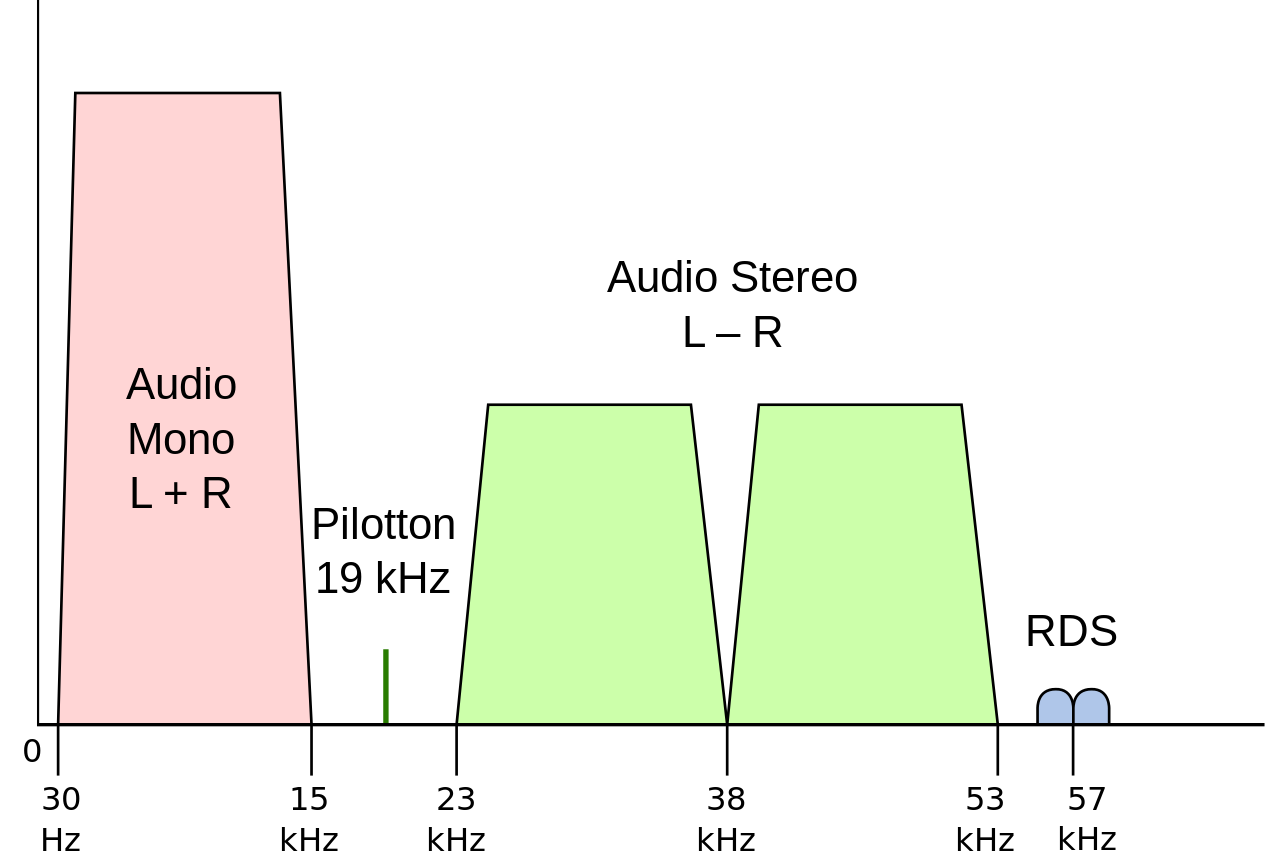
\includegraphics[width=9cm]{img/fm-channel-baseband.png}
  \caption{Allocation of frequencies in an FM channel \cite{ref_fig_channel_freqs}}
  \label{fig_channel_baseband_freqs}
\end{figure}

\subsubsection{Mono Audio Part}

The mono audio stream is located between 30 Hz and 15 kHz.
This signal is built by the sum of the left and right audio channels.
%The lower limit at 30 Hz is to prevent the transmission of a direct current (DC) part, which would require a large amount of power in transmission.
%This effect is one of the downsides of amplitude modulation (AM), where the carrier is located at the channels' center frequeny and requires a high transmission power. % TODO: check this fact
The upper limit at 15 kHz is chosen to maintain a sufficient spacing to the first subcarrier.

For audio streaming, as in FM broadcasting, this is not a limitation, since it is unlikely to have frequencies higher than 15 kHz in an audio stream.
Also, this already reaches the upper limit of the human ears' bandwith, so higher spectral parts will not be heard anyway.

\subsubsection{Pilot Tone}

The first subcarrier is allocated at an offset of 19 kHz from the center frequency.
This subcarrier is also called the 'pilot tone', since it is a continuous signal.
It is independent of any varying message signal content.
The pilot tone is used for stereo audio demodulation.
To regenerate a stereo audio signal, the left and right audio channels need to be recovered correctly.

\subsubsection{Stereo Audio Difference}

A signal that is constructed by the difference between the left and right audio channel is modulated on a 38 kHz subcarrier.
This subcarrier is an integer multiple of the pilot tone at 19 kHz, for practical reasons.
However, the 38 kHz carrier is suppressed and thus not visible in the received spectrum.
The modulation technique that is used for this spectral part is called dual-sideband suppressed-carrier (DSB-SC).
Even though the carrier is suppressed, it can still be recovered, because it is phase coherent with the 19 kHz pilot tone per definition.

The bandwidth for this difference-signal spans 15 kHz on either side of the subcarrier.
It is used to generate a stereo audio signal, in combination with the mono signal.
This process is explained into more detail in chapter \ref{sec_fm_sig_demod}.

\subsubsection{Additional Services}

Considering all these parts in the spectrum, there is still free bandwidth available to use up to the maximum channel bandwitdh of 100 kHz in one sideband.
Because of that, additional services were added to the pure audio transmission, to provide additional data services and information.

Services that were implemented are the Data Radio Channel (DARC), which is mostly used in Japan and the USA, the Subsidary Communication Authorization (SCA) and the Radio Data System (RDS) \cite{ref_rohde_u_schwarz}.
Out of these, RDS is the most significant service in Europe.
It is used to transmit additional information about the channel, such as the radio stations' name, the currently playing songs' title or traffic information.\\

\noindent
The information about the frequency spectrum was taken from \cite{ref_fm_broadcast_tutorial_and_basics}.

%%%%%%%%%%%%%%%%%%%%
\section{Algorithms for Digital FM Demodulation}
  %see literature/FmDemodulator.pdf (Sect. 3.3)
  %see literature/00476180 Digital FM Demodulator for FM, TV, and Wireless.pdf (Sect. II and III)

An FM signal that is received, for example from an antenna, needs to be demodulated in order to decode its actual data content.
In general, an FM demodulator serves the purpose to transform a frequency modulated signal (FM) into an amplitude modulated signal (AM), so that AM signal processing techniques can be applied afterwards.\\

The radio frequency antenna signal usually needs to be amplified, bandpass-filtered, and down-converted to baseband, using subsampling and quadrature-mixing, or similar strategies.
This part of the signal processing chain is assumed to be working correctly and is out of the scope of this chapter. %TODO: write up/down conversion in other chapter?
The FM signal that is evaluated here is assumed to be a quadrature-mixed signal in baseband, which means that inphase and quadrature (I/Q) signals are available.

%TODO: show downconversion path (maybe as a figure?)
%https://www.veron.nl/wp-content/uploads/2014/01/FmDemodulator.pdf

In the following sections, two digital FM demodulator variants are described.

% TODO: add img/discrimination_method_bd2.png here (?)

%%%%%%%%%%%%%%%%%%%%
\subsection{Frequency Discriminator}


A frequency discriminator can be defined as a black box component, that generates an output that is directly proportional to the frequency of the input FM signal.
Different strategies can be implemented in this black box component - the discriminator.
Here, a differentiator with a subsequent envelope detector is used, which is shown in Fig.\ref{fig_bd_freq_discriminator}.

\begin{figure}[!h]
  \centering
  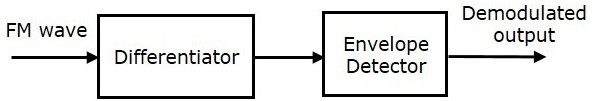
\includegraphics[width=7cm]{img/discrimination_method_bd1.jpg}
  \caption{Frequency discriminator block diagram \cite{ref_fig_freq_discriminator}}
  \label{fig_bd_freq_discriminator}
\end{figure}

% TODO: check which one i'm describing
%%%%%%%%%%%%%%%%%%%%
\subsubsection{this one}
%%%%%%%%%%%%%%%%%%%%
%\subsubsection{Baseband Delay Demodulator}
%%%%%%%%%%%%%%%%%%%%
%\subsubsection{Phase-Adapter Demodulator}
%%%%%%%%%%%%%%%%%%%%
%\subsubsection{Phase-Locked Loop (PLL)}
%%%%%%%%%%%%%%%%%%%%
%\subsubsection{Mixed Demodulator}

This type of demodulator converts the FM signal into an AM signal, but still leaves an FM content.
The transformation that happens here can be expressed in a formula, by simply differentiating Eq.\ref{equ_fm_func}.
This operation, with simple algebraic transformations, results in
\begin{equation}
  \frac{d s(t)}{dt} = A_c 2 \pi \Big[f_c + k_f m(t) \Big] sin \Big(\omega_c t + 2 \pi k_f \int m(t) dt -pi \Big)
  \label{equ:fm_demod_discriminator}
\end{equation}

An important requirement for the differentiator is, that the input signal is of a constant amplitude \cite{ref_schnyder_haller}.
The transmitted signal is subject to random additive noise on the transmission channel.
The differentiator would deliver wrong results because of this noise, when substracting two consecutive samples, as described in Eq.\ref{equ:differentiator_two_samples}.
To achieve a constant amplitude, the received complex baseband signal $s(t)$ can be normalized to a value of one.
\begin{equation}
  s_{norm} = \frac{s}{|s|} = \frac{A(n)\ e^{j\phi_{FM}(n)}}{|{A(n)\ e^{j\phi_{FM}(n)}|}} = e^{j\phi_{FM}(n)}
\end{equation}
\begin{equation}
  e^{j\phi_{FM}(n)} = |1|
\end{equation}

A differentiation in hardware is simply performed by substracting two consecutive samples, like
\begin{equation}
  \frac{d s(t)}{dt} = s(t) - s(t-\Delta t)
  \label{equ:differentiator_two_samples}
\end{equation}
where $\Delta t$ is the inverse of the sample frequency.\\ %TODO: check this (i'm using a 3-tap FIR in FPGA)

The differentiated signal Eq.\ref{equ:fm_demod_discriminator} consist of an AM and an FM content.
The FM part is described by the sine function.
The more important part is the AM part, which resembles the message signal.
It is described by the term within the square brackets.

The differentiated signal Eq.\ref{equ:fm_demod_discriminator} in time-domain is shown in the top left diagram in Fig.\ref{fig_time_domain_envelope_detect}.
This signal needs to be fed into an envelope detector, as seen in Fig.\ref{fig_bd_freq_discriminator}.
The envelope detector extracts the envelope by removing the high frequency portion.
The method implemented in Fig.\ref{fig_time_domain_envelope_detect} is one of the most simple ones and is usually referred to as 'Asynchronous Half-Wave Envelope Detector'\cite{ref_envelope_detector}.
It consists of a thresholding unit to remove negative values and a conventional lowpass filter.
In analog implementations, the thresholding unit is a diode.
The lowpass' cutoff frequency needs to be adapted to the envelope signals' maximum frequency, since it needs to be able to follow the signal, but also sufficiently smooth out the rectified signal.

Different methods may be implemented for the envelope detector.
For example, an 'Asynchronous Full-Wave Envelope Detector' can be used.
Therefore, the previous method only needs to swap the thresholding unit with an unit that calculates an absolut value.
In that architecture, a full-wave rectification is performed on the signal, which significantly improves the envelope detection accuracy \cite{ref_envelope_detector}.
The envelope is followed more exactly, because of the higher power that is available in the signal, since the entire signal is taken into account, and not only the positive half, as in the previous half-wave method.

\begin{figure}[!h]
  \centering
    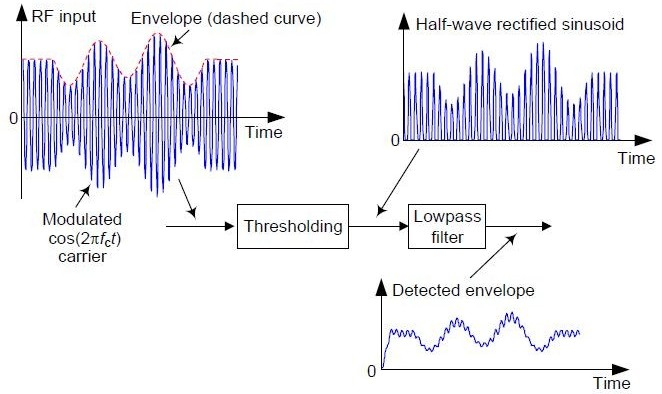
\includegraphics[width=8.8cm]{img/envelope-detect-time-domain.jpg}
  \caption{Time-domain signals in envelope detection \cite{ref_roppel}}
  \label{fig_time_domain_envelope_detect}
\end{figure}

%%%%%%%%%%%%%%%%%%%%
\subsection{Phase-Locked Loop}

A Phase-Locked Loop (PLL) can also be used to transform an FM signal to an AM signal.
A PLL is a feedback loop that is usually used to generate an output signal that has a fixed phase reference to its input.
In the case of FM demodulation, the loop filter in the feedback branch is configured to be able to follow the frequency variations on the input, which is directly related to the encoded information.
The output of the PLL directly delivers an AM signal, which corresponds to the transmitted information. \cite{ref_schnyder_haller}

FM demodulation with a PLL is not described into more detail, since this thesis is focussing on the concept of an entire system architecture.

%%%%%%%%%%%%%%%%%%%%
\section{Demodulation of Broadcast FM}

This chapter describes the demodulation of the information content of an FM broadcast channel, as it is used in commercial FM radio broadcasting.
The assumption here is, that the actual FM demodulation, as described in chapter \ref{sec_fm_sig_demod} is already done correctly.
A frequency spectrum of an FM channel is shown in Fig.\ref{fig_channel_baseband_freqs} above.

explaine multiplex signal somewhere

%%%%%%%%%%%%%%%%%%%%
\subsection{Mono}
\label{subsec:demod_mono}
  The first part of the channel frequency spectrum is the mono audio signal. It is summation signal of the left and right audio channel.
  A mono receiver can thus simply replay the so-called multiplex signal, which is generated by the FM demodulation described in chapter \ref{sec_fm_sig_demod}. The 19 kHz pilot tone will not be audible by most people, because it is outside of the range of a human ear. Besides that, any used speaker may also be unable to produce a frequency in this range. This explanation applies to several higher frequency components in the spectrum as well.
  In case the multiplex signal should be stored it in a file with 44.1 kHz samplerate, a lowpass with a cutoff frequency of 15 kHz and sufficient attenutation before 19 kHz needs to be inserted before the decimation and file output.

\subsection{Stereo}
  Demodulating an FM channel to recover a stereo audio signal requires a more sophisticated approach.
  In the channel frequency spectrum, there are two main parts of the audio signal - the sum and difference of the left and right audio channel signals.
  To combine these to a stereo signal, the following equations can be applied.
  \begin{equation*}
    L = (L+R) + (L-R) = (2)L
  \end{equation*}
  \begin{equation}
    R = (L+R) - (L-R) = (2)R
    \label{equ_stereo_from_sum_diff}
  \end{equation}

  The block diagram in Fig.\ref{fig_bd_stereo_demod} illustrates the signal processing chain for stereo audio. In the block diagram, $x(t)$ represents the multiplex signal from the FM demodulator. Signals $x_l(t)$ and $x_r(t)$ describe the left and right audio signal, respectively.

  \begin{figure}[!h]
    \centering
      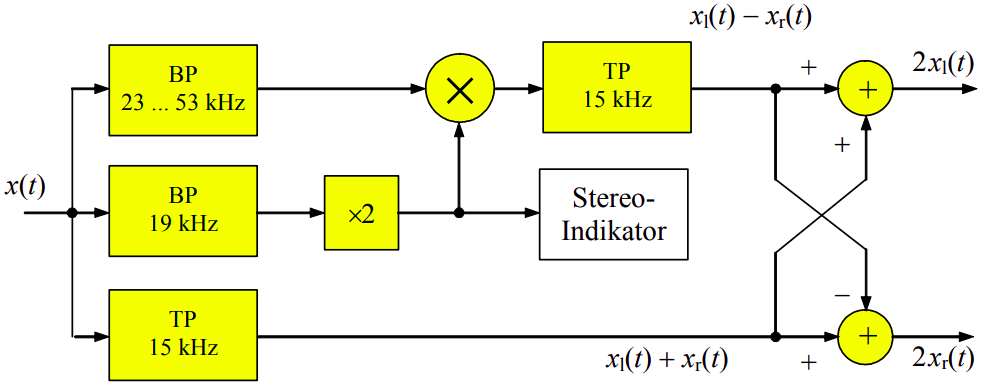
\includegraphics[width=8.8cm]{img/fm-demod-stereo-audio.png}
    \caption{Block diagram of FM stereo audio demodulation \cite{ref_roppel}}
    \label{fig_bd_stereo_demod}
  \end{figure}

  The central branch selects the pilot tone at 19 kHz with a bandpass filter.
  This bandpass needs to have a frequency response that is sharp enough to have a sufficient attenuation at $\pm$4 kHz, since this is where the summation and difference signals frequencies are allocated.
  Afterwards, the pilot tone frequency is doubled via a PLL to achieve a 38 kHz to later demodulate the difference signal phase-coherently.
  The PLL lock indicator can be re-used as an indicator, whether a pilot tone is existent.
  In the upper branch, a bandpass filter selects the difference signal with ranges from 23 to 53 kHz.
  It is then modulated to baseband by the previously generated 38 kHz subcarrier.
  Subsequently, a lowpass limits the signal to the audio signal bandwidth of 15 kHz.
  The lower branch lowpass-filters the summation signal.
  The rightmost part in the diagram performs the combination of summation and difference signals, according to Eq.\ref{equ_stereo_from_sum_diff}.


%%%%%%%%%%%%%%%%%%%%
\chapter{System Design Process}
\label{cha:SystemDesignProcess}

The process of system design is a central topic in the development of any product.
This chapter describes general techniques for system design.
However, they can also be directly applied to FPGA design.
Additionally, tools that are specifically used in FPGA design are introduced.

%%%%%%%%%%%%%%%%%%%%%%%%%%%%%%%%%%%%%%%%%%%%%%%%%%%%%%%%%%%%%%%%%%%%%%%%%%%%%%
\section{General}

The following sections describe a generalized approach to system design.
A process called SIMILAR is explained, as well as selected topics that are relevant.
The researched information for this section is mainly based on \cite{BahillA.Terry2017TDiS}.

%%%%%%%%%%%%%%%%%%%%%%%%%
\subsection{The SIMILAR Process}
%TODO: maybe include additional facts from https://slideplayer.com/slide/14327503/

The SIMILAR process provides a general approach to problem solving.
It can be applied to any kind of problem that can be of technical, as well as non-technical nature, in order to successfully achieve the specified requirements.
The concept was developed by A.T. Bahill and B. Gissing, who evaluated and compared multiple existing processes to find their similarities.\\

The acronym SIMILAR consists of the following components.

\begin{itemize}
  \item \textbf{S}tate the Problem
  \item \textbf{I}nvestigate Alternatives
  \item \textbf{M}odel the System
  \item \textbf{I}ntegrate Components
  \item \textbf{L}aunch the System
  \item \textbf{A}ssess Performance
  \item \textbf{R}e-evaluate
\end{itemize}

Each of these terms represents a separate step in the process diagram shown in Fig.\ref{fig:similar_process}.
The steps can be seen as iterative and parallel, as the process runs during the product development cycle.

\includepicture [0.95] [0] {The SIMILAR process in a graphical representation \cite{BahillA.Terry2017TDiS}.} {similar_process} {img/draw.io/similar_process}

%%%%%
\subsubsection{State the Problem}

The very first step of the process is to state the problem that is to be solved.
This can be the initial definition of a new product, but can also be the definition of an improvement that is to be made for an existing product.
Because of that, input for the problem statement can be generated by various parties, such as customers, product developers, regulatory agencies or manufacturers, just to name a few.
In the process diagram, all these possible input parties are labeled as stakeholders.\\

Generally speaking, the problem statement serves the purpose to build a common understanding of the problem between a stakeholder and the developer.
In case there is a mismatch, an engineer may spend valuable time to develop a sophisticated solution to a problem that was not even a requirement.
Thus, any time spent to develop this feature is worthless, which highlights the importance of a correct problem statement.\\

An important guideline for the specification of this problem statement is, that each requirement is descibed in the way of \textit{what} needs to be done, not \textit{how} it needs to be done.\\

The problem statement is updated and improved by the Re-evaluate step, which is described later.

%%%%%
\subsubsection{Investigate Alternatives}

In almost any kind of problem, there are multiple ways in order to achieve a successful solution.
However, some solutions may be preferred over others because of certain criteria that are evaluated.
Such criteria may be cost, risk, schedule or performance.
Based on the combined evaluation of these factors, a decision in favor of one selected alternative is made.
This part of the process is also called concept exploration.\\

It is important to note that this step is a repeated, iterative step.
This is necessary, since there may only be a few known facts available at the initial intestigation.
Further design steps, such as a first estimation of the intended design implementation, simulation results, or a prototype can provide more data and facts.
These can be used to re-evaluate the alternatives and consequently optimize the design process.


%%%%%
\subsubsection{Model the System}

Based on the previous steps, a model for the system is developed here.
This includes a process model, that is used for stragetic planning towards cost reduction, optimization of the implementation effort, or the schedule of subprojects, and a product model, which supports trade-offs and the identification of risks, or helps to explain the system as a whole.\\

Typically, a coarse model is created for almost all alternative designs that were found in the previous step.
A more detailed model is developed for the single, selected design.
The model itself may be represented in many different ways, such as state machines, block diagrams, flow diagrams, simulations or object-oriented diagrams.

%%%%%
\subsubsection{Integrate Components}

This step combines multiple single components into a larger, integrated system, which can then be treated as a whole.
In order to be able to do that, interfaces between the components and subsystems need to be defined.
Optimally, these interfaces are designed in a way that the amount of data that needs to be exchanged is kept to a minimum.
It is of advantage, if a subsystem only transfers finished products that it produced to another subsystem.
The aim to develop simple interfaces is of special advantage in systems that include a feedback loop.
There, managing the feedback loop connections is easier if there is a clear interface, so the loop can be connected around an entire subsystem, instead of interconnecting within the subsystems.

%%%%%
\subsubsection{Launch the System}

The system launch actually runs the system in a defined environment, so that it can perform what it is intended and designed to do.
The defined environment can be the final, operational environment, or just a simulation which provides an output that is detailed enough for an evaluation.
In a product that involves hardware development, this step may include the installation of commercial off-the-shelf products with a modified prototype software.
However, since the SIMILAR process is applicable for any kind of problem, this might also be a business process, where the launch step may be the roll-out of the subprocesses and tasks in the respective departments of a company.

%%%%%
\subsubsection{Assess Performance}

This step is all about measurements.
The performance of a system can only be evaluated, if it can be measured by using different metrics.
Evaluation criteria are used, based on the measurements of the technical performance, which can help to find trade-offs or to mitigate risk in design and manufacturing.

%%%%%
\subsubsection{Re-evaluate}

The re-evaluate step is a central building block in the SIMILAR concept.
All of the other steps have a connection to it, in the form of a feedback loop.
However, depending on the nature of the project and the point in the timeline of its life cycle, not all of these loops may be exercised all the time.
The idea of re-evaluation and the subsequent improvement of a process is a widely applied and well-known concept.
Its main function is to observe an output and to use this information to improve the systems' input.

%%%%%%%%%%%%%%%%%%%%%%%%%
\subsection{Design for Reuse}

A design principle that is often used is design for reuse.
It enables a faster and more efficient development of products, which leads to an overall decrease in development cost.
Additionally, the product is likely less error-prone, since the reused parts of the system are already tested at this point.
After all these positive arguments, there is a counter argument to it, though: designing a system with reuseable subsystems comes with cost.
Additional effort is required to design the subsystems in a way so that they can be reused in another project.
However, this additional effort may potentially already be paid off, when a single subsystem can be reused in a future product and thus, it is worth the effort.

%%%%%%%%%%%%%%%%%%%%%%%%%
\subsection{Validation and Verification}
\label{sec:ValidationAndVerification}

The terms validation and verification are closely related, but have a different meaning in system design.
Verification tests the properties of the developed product against the previously determined specification and requirements.
It stives to build the \textit{system right}.
Validation on the other hand tries to build the \textit{right system}.
It proves that the product does what it is intended to do.
This is important in order to develop the product according to what the customer actually needs.
To avoid to divert from these customer needs, validation is done throughout the products' development cycle, from the beginning to the end.
Various artifacts can be collected during the process, in order to have a traceable documentation of the decision that were made.\\

Validation may also fail, which means that the chosen system may be the wrong system for the respective customers needs.
As an example, the system may be very sensitive to variations of a parameter that a customer cannot influence.
Another example is when a system is more sensitive to certain parameters than to its inputs.
In both cases, the system may be the wrong system for the specific problem and should urgently be re-evaluated.\\

In order to expose such failures as early as possible, any test engineer should be instructed to always keep an eye on the process of validation, which means to check if the team is building the \textit{right system}.
Therefore, a test engineer should be familiar with the problem statement.

%%%%%%%%%%%%%%%%%%%%%%%%%%%%%%%%%%%%%%%%%%%%%%%%%%%%%%%%%%%%%%%%%%%%%%%%%%%%%%
\section{System Design Targeting FPGAs}

A wide range of system-level design approaches are available that are targeting FPGAs.
In this section, some selected approaches are described.
The research for this section is mainly based on \cite{GesslerRalf2014EES}.

%%%%%%%%%%%%%%%%%%%%%%%%%
\subsection{V-Modell}

The development of a product requires an organized approach, in order to successfully achieve the requirements.
The common term for such an organized approach is the process model, which represents a guideline on how to organize and structure the development cycle.\\

A well-known process model is the so called V-Model.
It is based on the similarly well-known Waterfall Model, and has its name because of the distinct V-shape of its process diagram, as it is shown in Fig.\ref{fig:v_modell}.
One of the main characteristics of the V-Model is, that one phase needs to be completed before the following phase can start.
This classifies the model as a static process model and is one of the main disadvantages at the same time, because it makes the model inflexible to adaptions of the requirements.
The advantages however are that it is easy to install and apply, each phase has its specific deliverables, good results can be achieved for large projects with simple requirements and the early test phases.\\

The disadvantages of inflexibility towards changes of requirements and the fact, that it is difficult to consider all all eventualities in the creation of the V-model, led to the innovation of modern process models, which are iterative and thus more flexible.\\

The V-model applies to general software development, or project development, but can directly be mapped to FPGA development.
The model is covered in this thesis section, because it shows the clear testing structure of module tests (unit tests), integration tests and system tests, which is especially important in projects that target hardware, such as FPGA projects.\\

Furthermore, the V-model diagram in Fig.\ref{fig:v_modell} shows the difference between validation and verification, as it is explained in the previous section \ref{sec:ValidationAndVerification}.

\includepicture [1.0] [0] {The V-Modell process diagram \cite[Abbildung 3.5]{GesslerRalf2014EES}.} {v_modell} {img/draw.io/v_modell}

%%%%%%%%%%%%%%%%%%%%%%%%%
\subsection{High-Level Synthesis}

High-Level Synthes (HLS) is an FPGA design methodology that provides a high level of abstraction, and thus can be seen as a system level design method.
Different languages are used for HLS - two well-known languages are SystemC, which is a library for \cplusplus\ to provide modelling and simulation features, and plain \cplusplus.
A comprehensive list of available HLS tools and languages can be found in Section 3.3 of \cite{2016FfSP}.\\

The main idea of HLS is, that the hardware design can be written in abstract modules, that represent the actual functional meaning of a feature or algorithm, rather than the complex, low-level hardware details.
HLS achieves this by allowing to develop the code in a high-level language, such as \cplusplus.
This high-level code is then automatically transformed into hardware description language (HDL) by the respective HLS tool.\\

In this thesis, only the HLS of plain \cplusplus\ is covered.
SystemC is not discussed, since it may potentially be less important in the future.
In the latest Xilinx HLS tools 'Vitis HLS' and 'Vivado HLS', the language SystemC is already deprecated \cite{VivadoHlsSystemC}.\\

\noindent
HLS is described into more detail in Chapter \ref{cha:HLS}.


%%%%%%%%%%%%%%%%%%%%%%%%%
\subsection{Direct Implementation}

The implementation of low-level hardware description language (HDL) in the register transfer level (RTL) is denoted as 'direct', or 'manual' implementation in this thesis.\\

Two commonly used languages therefor are VHDL and Verilog.
Both have similar features to describe hardware in the signal level, with parallel structures and timing-dependent architectures.
The languages can describe a design in a hierarchical order, so that the separate modules can be constructed in a way that an overview of the functionality of the system remains given.
Synthesis, as well as simulation is supported, which allows efficient development of RTL designs.\\

%%%%%%%%%%%%%%%%%%%%%%%%%
\subsection{Implementation with Tool Support}

The implementation of FPGA designs with tool support focuses on the development as a model-based approach, that is often featured by a graphical programmers interface.
This is often used for prototyping in an early phase of product development.
A well-known example for such a model-based approach is Matlab, and its graphical tool Simulink.\\

Matlab can be used to describe and develop hardware-oriented algorithms, since it supports various library functions, such as the fixed point representation of numbers.
A major advantage is, that fast prototyping of an algorithm, as well as a fast simulation of the system is achievable.
Simulink is a graphical editor, that allows to connect functional blocks in a block diagram and create a system in that way.
Multiple toolboxes support additional blocks, that abstract complex functionalities, so that a fast prototyping is possible here as well.\\

A powerful feature of Matlab and Simulink is, that it can be used similar to an HLS tool.
Matlab code, as well as Simulink block diagrams can be transformed into low-level RTL code for an FPGA design.

%%%%%
\subsubsection{Simulink System Generator}

A full system-level design approach can be covered with the Simulink System Generator.
This includes the high-level development of the system as a block diagram in Simulink, the automated generation of low-level RTL code for the FPGA hardware, and the verification in simulation and in hardware, in the form of hardware-in-the-loop.
This workflow is supported for Xilinx FPGAs and is specifically targeting system design engineers, who work in rapid prototyping to generate hardware utilization estimates for the final products' hardware.\\

Fig. \ref{fig:simulink_system_generator} shows this entire design approach in a block diagram.
The abbreviation ISE stands for Integrated Software Environment, and is Xilinx' development environment that includes the FPGA synthesis tool.

\includepicture [0.8] [0] {Overview of the capabilities of the Simulink System Generator \cite[Abbildung 5.11]{GesslerRalf2014EES}.} {simulink_system_generator} {img/simulink_system_generator}

%%%%%
\subsubsection{Simulink HDL Coder}

The Simulink HDL Coder tool can generate VHDL or Verilog code from Matlab functions or Simulink block diagrams and state diagrams.
The generated code can be used in Xilinx, as well as Intel/Altera FPGA hardware.
This allows prototyping of algorithms, while continuously having detailed information of the target implementation, such as an estimate of the hardware logic utilization, or even the critical path in the logic.

%%%%%%%%%%%%%%%%%%%%%%%%%
\subsection{Level of Abstraction}

Multiple implementation methods are introduced in above sections, which all have different levels of abstraction.
VHDL and Verilog require, or allow, a very detailed description of the RTL code, while SystemC, \cplusplus, or Matlab and Simulink provide a high level of abstraction.
In Fig.\ref{fig:fpga_design_levels}, the various implementation methods are compared, with their respective levels of abstraction.\\

In conclusion, it is an engineers' choice which implementation method to use in order to develop a product.
A trade-off between optimization and the level of abstraction is likely to be made.
The decision may not always be obvious, but should be based on the fundamental requirements of the final product.

\includepicture [0.5] [0] [H] {Abstraction levels of the different implementation languages \cite[Abbildung 5.1]{GesslerRalf2014EES}.} {fpga_design_levels} {img/fpga_design_levels}

%%%%%%%%%%%%%%%%%%%%%%%%%%%%%%%%%%%%%%%%%%%%%%%%%%%%%%%%%%%%%%%%%%%%%%%%%%%%%%
\chapter{High-Level Synthesis}
\label{cha:HLS}

This chapter covers High-Level Synthesis in general, but also describes details that specifically apply to Xilinx.
The main sources of information for this chapter are found in \cite{VivadoUgHLSIntro}and \cite{VivadoUgHLS}.

%%%%%%%%%%%%%%%%%%%%%%%%%%%%%%%%%%%%%%%%%%%%%%%%%%%%%%%%%%%%%%%%%%%%%%%%%%%%%%
\section{Introduction}

In software development, engineers are used to writing code in a high-level language, such as C or \cplusplus.
With these languages, specific hardware details are abstracted and thus, very little knowledge of the target hardware is required.
The compiler takes over these details as it transforms the code by using the underlying, supported instruction set of the target hardware.
This has been the standard for many years by now.
In the earlier times however, it was common practise to develop programs in the low-level assembly language.
The supported instruction set of the target CPU had to be implemented directly by the software engineer.\\

A direct comparison can be drawn to FPGA design.
An FPGA engineer historically develops code in the register-transfer level (RTL), which is common practise until today.
This can be compared to developing software in the assembly language.
However, the recent development towards automation and code generation brought up High-Level Synthesis (HLS).
There, the FPGA design can be described in a high-level language, such as C or \cplusplus, which is convenient and allows to focus on the algorithm, rather than hardware details.
This high-level code is then transformed into the low-level RTL automatically, by the HLS tool.\\

The usage of HLS tries to bring software- and hardware development closer together and tries to make these two worlds more similar.
In software development, there are different compilers for multiple processor architectures, which can be used to port a program to another target hardware.
The idea of HLS is to create the same level of abstraction - write code in a high-level language, which is agnostic of its target hardware architecture.\\

A major achievement in the usage of HLS is the shorter development time.
The time that it takes to develop a first working version of the intended design can be significantly reduced, compared to the development in RTL code directly.
This is especially important when an FPGA design is combined with a software part, like in a System On Chip, since software development is comparably fast.
Fig.\ref{fig:timeline_performance_first_prototype} schematically displays the difference in development time, over performance and degree of optimization, when the same functionality of a prototype is implemented in different methods for various targets.
The compared targets are an x86 processor CPU, a digital signal processor (DSP), a graphics processing unit (GPU) and the FPGA design in RTL or HLS implementation.
It is clearly visible, that the FPGA design with the HLS design approach achieves a first working prototype much earlier than the direct RTL approach.

\includepicture [0.8] [0] {Design Time vs. Application Performance, if the same functionality is implemented in different methods for various targets \cite[Figure 1-1]{VivadoUgHLSIntro}.} {timeline_performance_first_prototype} {img/timeline_performance_first_prototype}


%%%%%%%%%%%%%%%%%%%%%%%%%%%%%%%%%%%%%%%%%%%%%%%%%%%%%%%%%%%%%%%%%%%%%%%%%%%%%%
\section{State Of The Art}

Information for this section is found in \cite{EvolutionOfHLS}, \cite{XilinxVivisHLSOpenSource} and \cite{CompareHlsVHDLArticle}.\\

HLS has been developed over 20 years ago, but has not been able to replace the manual, traditional implementation of RTL, using VHDL and Verilog, so far.
Unfortunately, no published numbers about the market share of HLS in relation to traditional implementations could be found during the research in this thesis.
However, according to the given sources it is becoming more and more popular in recent years.
This is mainly based on the fact that the HLS tools keep producing results of better quality as they are developed further.
This especially regards the efficiency of the produced RTL code, the useability of the tools, as well as the better understandable correlation between the high-level code and the generated RTL code.\\

Xilinx is the largest manufacturer of FPGAs globally and therefore its tool 'Xilinx HLS' is widely used.
Intel, the second largest FPGA manufacturer, also has its HLS tool called 'Intel oneAPI' \cite{IntelHLSOneAPI}.
Both companies are conducting serious effort to push the HLS implementation method.
Xilinx recently open-sourced the code for the front-end of their HLS compiler.
The front-end processes the HLS code, specifically \cplusplus, and creates an intermediate representation from it.
The company expects to expand the community engagement and the encouragement of innovation, driven by users, with this step.
Also Intel with its oneAPI toolkit is trying to introduce a wider usage of HLS to the community.\\

In terms of language support, several tools settle for \cplusplus.
Intel oneAPI uses library APIs and DP\cplusplus\ (Data-Parallel \cplusplus), which is an extension to the ISO \cplusplus\ standard.
Xilinx also decided in favor of the \cplusplus\ language for their tools 'Vivado HLS' and 'Vitis HLS'.
In older versions, SystemC was supported for synthesis as well, but is now deprecated in the respective latest versions \cite{VivadoHlsDeprecatesSystemC}.\\

Summing up, HLS is gaining more and more attention as it becomes more efficient.
Its usage is being promoted and pushed forward with serious effort by the major FPGA chip manufacturers and tool vendors.

%%%%%%%%%%%%%%%%%%%%%%%%%%%%%%%%%%%%%%%%%%%%%%%%%%%%%%%%%%%%%%%%%%%%%%%%%%%%%%%
%\section{Functionality}
%
%transform high-level code to HDL.\\
%-analysis\\
%-scheduling\\
%-pipelining\\
%
%- Limitations\\
%dynamic memory allocation, etc.


%%%%%%%%%%%%%%%%%%%%%%%%%%%%%%%%%%%%%%%%%%%%%%%%%%%%%%%%%%%%%%%%%%%%%%%%%%%%%%
\section{Workflow}
\label{sec:hls:workflow}

This section describes the workflow for Xilinx HLS, as it is recommended in the user guide \textit{Introduction to FPGA Design with Vivado High-Level Synthesis} \cite{VivadoUgHLSIntro}.\\

Generally, as the user guide states, the quality and the correctness of the generated output can only be as good as its input.
Consequently, it is very important to follow the design recommendations and adhere to specific rules in order to produce a high-quality input software.\\

The following list presents the main steps that are required in the implementation workflow of an HLS IP core project.\\

\begin{itemize}
  \item \textbf{Software Testbench}\\
      The developed HLS IP code needs to be verified and checked for correct functionality in a software testbench, before it gets processed to RTL code.
      This can be done by using using conventional software development tools.
      Xilinx specifically recommends dynamic code checker tools like \textit{valgrind} or \textit{Coverity}.
      They support a developer in finding memory leaks, out-of-bounds memory access, uninitialized variables and similar issues.
      Furthermore, the application of code coverage tools like \textit{gcov} is recommended as well.
      In that way, the percentage of executed code lines of testbench and HLS code can be measured, to ensure a sufficient level of testing.
      The software testbench is also called 'C Simulation'.\\

      The implementation of the HLS IP code is subject to restrictions.
      As an example, dynamic memory allocation is not supported, since the entire code must be analyzable at runtime to be processed into RTL code.
      %For further details, please read the user guides regarding Xilinx HLS.
      In contrast, the testbench code does not have any restrictions.
      Anything that is supported in C/\cplusplus\ may be used here.\\

  \item \textbf{Co-Simulation}\\
      Co-Simulation serves the purpose to verify the correct functionality of the generated RTL code.
      It is not the goal to verify the algorithm, though.
      This is already done in the previous C simulation step.
      However, the issue is that the C simulation is executed like a regular program, which means it is executed sequentially, instruction by instruction and thus parallelism cannot be represented.\\

      This is where the Co-Simulation becomes neccessary.
      The RTL code is simulated with an HDL simulator software, which can actually simulate the parallelism as it exists in the FPGA hardware.
      In that way it can be ensured, that the user did not break the functional correctness of the algorithm, by giving wrong parallelization guidance to the HLS tool.\\

      The external simulator software has to run the complex HDL simulation and return data results, which is a time consuming task.
      Therefore, the execution time of this simulation type is expected to be approximately 10.000 times slower, compared to the C simulation.\\

  \item \textbf{Integration of the generated IP}\\
      At this point, the developed HLS code is fully verified and can successfully be transformed into working RTL code.
      Xilinx HLS exports the generated RTL code in an IP structure that is supported by its IP integrator tool, that is used in Vivado or Vitis.
      Therefore, the developed IP core can be imported to the block design as another processing block, get connected with other IPs, and in that way get integrated into a larger design.\\

  \item \textbf{Synthesize FPGA bitstream}\\
      Like in any other FPGA development cycle, the created block design can now be synthesized.
      This generates a bitstream file, which can be programmed into an actual FPGA hardware.
      Depending on the architecture of the system, the developed IP may now interface with the on-chip CPU, in the example of a System-On-Chip.\\
\end{itemize}

These steps represent the standard workflow for the development of an integrated HLS IP.
A successful deployment on hardware can be achieved if they are completed accurately.
There may be more and deeper knowledge necessary, in order to use this design approach.
This thesis however focuses on system design, not on HLS specifically, and thus a comprehensive study of the referenced literature is recommended.

%%%%%%%%%%%%%%%%%%%%%%%%%%%%%%%%%%%%%%%%%%%%%%%%%%%%%%%%%%%%%%%%%%%%%%%%%%%%%%
\section{Coding}

This section gives a brief overview of some HLS-specific \cplusplus\ features that are supported with Xilinx tools.
More detailed information can be found in the respective user guide \cite{VivadoUgHLS}.

%%%%%%%%%%%%%%%%%%%%%%%%%
\subsection{Data Types}

HLS supports special data types, which are not available in standard \cplusplus.
The focus of these data types is mainly to support an optimized translation into RTL, which requires the least amount of logic cells in the FPGA.\\

Standard \cplusplus\ only supports variables in the bitwidth of byte-boundaries, so in multiples of 8 bit.
However, this may be inefficient to fit into the available FPGA target hardware.
One example therefor is the DSP48 macro that Xilinx FPGAs have built-in.
They support the multiplication of only up to 18 bit.
In an example application, the reachable number range of a variable might be limited to 17 bit for the multiplication.
However, in order to represent that, using a 32 bit data type would be necessary in standard \cplusplus.
The HLS compiler does not have this prior knowledge of the number range limit and would thus implement a 32 bit multiplication, which is a waste of resources in this case.
Because of this reason, a major feature of HLS is the possibility to define data types with arbitrary bitwidths.
In that way, the above example can be optimized to use a data type that has a bitwidth of 17 bit, which is exactly the bitwidth that is required for the application.
This results in a lower logic utilization, which in turn results in a higher maximum clock frequency that can be used.
Consequently, more functionality an be implemented in the FPGA device.
The referenced user guide shows a design example where an area reduction of 75\% is achieved by just reducing the bitwidths.\\

The argumentation is equally valid for integer data types, as well as fixed point data types.
In calculations it is often necessary to represent fractional numbers.
In standard \cplusplus, floating point data types are used therefor.
However, floating point operations require a large amount of logic to implement and thus, HLS provides fixed point data types.
These can be instantiated in arbitrary bitwidths, where integer and fractional bitwidths can be specified separately.
The fixed point format is often described in the format 'integer.fractional', like '2.14', which represents a 16 bit fixed point data type that has 2 integer bits and 14 fractional bits.\\

An example for the usage of integer and fixed point data types is given in the following code section.

\begin{CppCode}
  #include <ap_int.h>
  #include <ap_fixed.h>

  ap_int<9>   custom_integer_var1;         //  9 bit integer, signed
  ap_uint<17> custom_integer_var2;         // 17 bit integer, unsigned

  ap_fixed<16,2>  custom_fixedpoint_var1;  // 16 bit fixed point, 2.14 format, signed
  ap_ufixed<14,4> custom_fixedpoint_var2;  // 12 bit fixed point, 4.10 format, unsigned
\end{CppCode}

%%%%%%%%%%%%%%%%%%%%%%%%%
\subsection{Interfaces}

%%%%%%%%%%%%%%%%%%%%%%%%%
\subsection{Compiler Directives}

e.g. \#pragma's

%%%%%%%%%%%%%%%%%%%%%%%%%
\subsection{Optimization}

%\subsection{Functions}
%\subsection{Loops}
%\subsection{Conditional Statements}

%%%%%%%%%%%%%%%%%%%%%%%%%%%%%%%%%%%%%%%%%%%%%%%%%%%%%%%%%%%%%%%%%%%%%%%%%%%%%%
\section{Testbench}

The general significance of the simulation testbench for a HDL design is explained here, as well as the different levels of abstraction in which a HLS testbench can be executed.
These different levels of abstraction in the testbench execution are a major difference between a VHDL testbench and an HLS testbench.
The most important impact thereof is the execution speed - the time it takes to simulate a number of test cases on the DUT.\\

Section \ref{sec:hls:workflow} above already mentioned the topics of testbenches and simulation types.
The following descriptions shall be seen as a comprehensive extension around these topics.

%%%%%%%%%%%%%%%%%%%%%%%%%
\subsection{General}
\label{sub:hls:testbench:general}

In the development of software that runs on a CPU, the tool of step-by-step debugging is commonly used during the development process.
Various verification and testing libraries exist, in order to create unit tests, for example.
The advantage is, that the code that is developed there, can be compiled and run on the target CPU directly, while maintaining the direct instruction-by-instruction representation of the code.\\

However, in the development of hardware with any HDL, this is not possible.
HDL languages provide a syntax and semantic representation that allow to create parallel structures and a dependency on timing, such as a system clock.
The design is based on signals that perform logic operations and transfer values into registers.
Thus, HDL code is often called register-transfer level, or short, RTL code.
Before this code can be run on the target hardware, i.e. an FPGA, it needs to run through a process called synthesis.
In synthesis, the HDL code is translated into a netlist and is consequently mapped into hardware logic cells that are available in the target device.
Various optimizations are done during this process, so that the direct connection to the code representation is lost.
Additionally, it is impossible to access every single signal within the design during debugging on the hardware, which is probably also one of the main issues.
Synthesis tools like Xilinx Vivado provide support to make debugging possible in hardware, but require a large effort to implement them, especially in terms of synthesis time.
Another big factor that speaks against debugging in hardware generally, is that the process of synthesis takes a comparably large amount of time to transform code into the target technology.
Each time the code is adapted, the entire synthesis process needs to be started over again.
Because of all of these reasons, debugging HDL code step-by-step as in software is not possible.\\

Thus, in order to allow debugging and verification of HDL code, the technology of simulation was invented.
Here, the HDL is also translated into a netlist that represents all the parallel processes just like in hardware, but the subsequent step of synthesis is not taken.
Therefore, simulation comes to a result much faster.
Since HDL designs actually only consist of electrical wires and some basic block primitives, like flipflops or lookup tables, it is difficult to verify correct values.
They would need to be compared in their binary bit-pattern format, at the correct point in time.
Of course the HDL language provides support with different datatypes, that abstract the binary number representation and make the numbers human-readable.
However, it remains an enormous effort to manually write testing code to verify a bus interface, for example.
In order to simplify such complex operations, various testbench frameworks and libraries are available to developers.

%%%%%%%%%%%%%%%%%%%%%%%%%
\subsection{C Simulation}

In C Simulation, the HLS compiler is used to create an executable binary that includes the testbench code, as well as the IP design of the DUT.
This binary can be run just like any other program.
The most important note here is, that the HLS code is \textit{not} transformed into RTL at this point.
Instead, the HLS code is treated as a regular \cplusplus\ code, that uses some libraries, like the fixed-point library.
This means, that the HLS IP cores' top-level function is used as a regular function call in the testbench.\\

The main advantage of this type of simulation is the major increase of execution speed.
The reason for this speed-up is the abstraction of timing, such as clock cycles or similar constraints.
In fact, there is absolutely no timing information that needs to be taken into account in this simulation.

%%%%%%%%%%%%%%%%%%%%%%%%%
\subsection{C/RTL Co-Simulation}

This type of simulation actually transforms the HLS IP code into RTL code, such as Verilog or VHDL, for the testbench.
This is done in three steps.\\

\begin{itemize}
  \item \textbf{Create input vectors}\\
  In this first step, the above explained, regular C simulation is executed.
  Hereby, the inputs that are sent to the DUT are stored as 'input vectors'.

  \item \textbf{Perform RTL simulation}\\
  Next, the previously generated input vectors are applied to the DUT.
  At this point, the DUT is already translated into RTL code, so the code that is used here is either VHDL or Verilog code.
  The default simulator is the Vivado Simulator (XSim).
  However, various other simulators like ModelSim are supported.
  The generated outputs of this step are stored as 'output vectors'.
  \item \textbf{Verify the results}\\
  The final verification step sources the output vectors back to the C testbench, which compares the outputs with the expected results.\\
\end{itemize}

\noindent
This type of simulation takes a significantly longer time to execute, because timing information now actually needs to be considered for the RTL code.

%%%%%%%%%%%%%%%%%%%%
\chapter{System Architecture and Concept}
\label{cha:SystemArchitectureAndConcept}

This chapter introduces the FM radio receiver project that is implemented as a major part of this thesis.
It specifically talks about the system level approach that is taken in the implementation of the project.
The main concept, as well as the architecture are explained.

%%%%%%%%%%%%%%%%%%%%
\section{Overview}

In the development of a project that includes multiple functional parts, it is always of advantage to start with a system level overview.
Major decisions can be made at this stage, before any implementation has begun.
This can have a direct impact on the efficiency of the entire development, which concequently has an impact on the final quality of the product.
A thorough system level design can also prevent from issues that would otherwise arise while the development is already ongoing.
As an example it could turn out that one of the functional parts is not able to fit into the integrated system, in the way it is implemented.
This leads to the necessity to re-engineer this entire functional block.
As a result, it takes more effort to implement the functionality, which directly correlates with the development cost and the time-to-market, in order to deliver the final product.
Summing up, a comprehensive system level architecture and concept can pave the way for a successful implementation of a project from start to finish.\\

In order to create a system level design, considerations around the high-level, final goal of the product are a good starting point.
This includes the definition of its functional range.
Once this is done, the target system or target hardware should be considered, because there are various ways to implement a certain functionality.
All of these variants will eventually result in the same output, but will, however, heavily differ in their implementation effort, efficiency, or their applicability for the products' aim in general.
Thus, things like the available hardware platform, implementation time, degree of optimization, output quality, and similar things are important factors at this stage.
Of course, there are many more factors to consider when a product is to be developed.
However, only a subset of these is covered here, since this chapter is focused on how this thesis' accompanying project was developed and is thus written in that context.\\

%%%%%%%%%%%%%%%%%%%%
\section{The project}

The aim of this thesis is develop a system architecture and concept, that allows the implementation of an FM radio receiver in multiple different ways, while providing an elegant way to compare the different solutions.
The final goal thereby is always be the same, that is: Listen to the music of a radio station that is transmitted over FM broadcast radio.\\

\noindent
A very high-level overview of the entire system is given by the block diagram in Fig.\ref{fig:bd_system_overview_highlevel}.
It shows the front end, which processes the received antenna signal, so that it can be used in the FM radio receiver block.
The radio receiver itself is implemented in multiple different variants.
The produced audio output is sent to a speaker, since the ultimate goal is to listen to a radio stations' audio signal.

\includepicture [1.0] [0] [H] {High-level overview of the system.} {bd_system_overview_highlevel} {img/draw.io/bd_system_overview_highlevel}

In the context of a system level design approach, several steps are necessary to find a solution that is ready to be implemented.
As a very first step, the inner workings of an FM receiver need to be understood.
This mainly regards the signal processing theory, to be able to decode the signal that is received by the antenna.
Chapter \ref{cha:SignalProcessingTheory} describes this part into detail.

As already mentioned above, multiple ways of technology and implementation can lead to a similar result.
Thus, the next step is to define a set of possible ways which will actually be implemented.
For this thesis, the decision was made to implement the FM radio receiver by using the following methods.

\begin{itemize}
  \item \textbf{GNU Radio}\\
      GNU Radio is a free and open-source software development toolkit to implement a software-defined radio.
      The implementation is done by connecting functional blocks in a block design.
      This abstracts the inner workings of each functional block and thus provides an implementation approach on a very high level of abstraction.
      GNU Radio supports interfaces to external RF hardware \cite{SoftwareGnuRadio}.
  \item \textbf{Matlab}\\
      Matlab is a software platform that can work with matrices and compute numerical solutions.
      Matlab also includes various toolboxes, that support developers with complex calculations and tasks on datasets.
      This includes a range of toolboxes for signal processing, such as filter designers or FFT functions, as well as convenient ways to visualize data \cite{SoftwareMatlab}.
  \item \textbf{FPGA: \cplusplus High-Level Synthesis}\\
      In order to use an FPGA, a hardware design needs to be developed for it.
      This can be done using high-level synthesis.
      High-level synthesis (HLS) is explained in detail in Chapter \ref{cha:HLS}.
  \item \textbf{FPGA: VHDL}\\
      Similar to the HLS approach, this is a variant to write a hardware design for an FPGA.
      The language VHDL is used in this approach.
\end{itemize}

In order to implement an FM radio receiver, all of the listed methods require deep knowledge about the neccessary details of signal processing.
However, the implementation of the various different methods require more or less knowledge and effort on the exact underlying implementation of each signal processing part.
This depends on their respective level of abstraction.

%-  implementation of a model and DSP concept in Matlab \\
%-  implementation in VHDL and HLS \\
%-  both use the same testbench source \\
%-  both are integrated into FPGA
%-  the FPGA output is read back into the firmware, for analysis \\

%%%%%%%%%%%%%%%%%%%%
\section{System concept}

The overall system concept has to be developed in a way, to fit the respective projects' needs and requirements.
There should be a clear structure, in order to help to create a working system successfully.
This structure should include a description of the data source, the data processing blocks and stages, commonly used parameters, as well as a strategy to verify the correct functionality of the system.
A good system structure tries to share as many parts as possible in the system.
This is to minimize the points of failure, as well as to reduce the effort of implementation.\\

In the apparent projects' case, a single block of the system is implemented in multiple ways, which should, however, all compute an equal output.
Thus, it is of advantage to define the data source to be common for all of these variants, to create a unified situation at the input.
Additionally, the data source may be chosen to be recorded, to have a known, reproducable set of input data.
This significantly eases the verification of the functionality in the final step, since all variants are expected to create the same output in the optimum, fully functioning case.
Not only the data source is important to be common, but also the way of verification.
In order to achieve that, the verification block needs to be able to compare multiple data outputs with the verification data, which is chosen to serve as the reference.\\

An example of a system concept and its architecture is developed and shown in Fig.\ref{fig:bd_system_overview_detailed}.
Here, a common data source is provided by the block called \textit{Front End}.
It records data from an antenna and saves it to a file, in a format that the consequent blocks require at their input.
Therefore, a reproducable input is ensured.
Within the \textit{FM Radio Receiver} block, all the different implementation variants are shown in parallel.
They all work on this common input source and generate their respective output.
This output data is again written to a file.
Hereby it is important to note, that the output of the \textit{Matlab} implementation is chosen to be the 'golden reference model' of correct output.
Its output is used as the verification data later in the process.
This is because Matlab was used to research decoding algorithms and to develop the DSP chain, which is used in the GNU Radio, HLS and VHDL implementations.
In addition to the verification data, the Matlab model also writes common parameters to a file.
These parameters are directly used in the other implementations, to ensure a common setup.
The final block is the \textit{Verification} entity, which compares the output files of all the variants, with respect to the chosen model parameters.\\

A major point in this system concept is, that it works independently of the respective implementation methodology.
This is especially important, since there is no possible way to run all these different variants in a single verification environment.
Instead, each methodology writes an output file, which is a supported functionality that is available anywhere.

\includepicture [1.0] [0] {Block diagram of the overall system concept.} {bd_system_overview_detailed} {img/draw.io/bd_system_overview_detailed}


%%%%%%%%%%%%%%%%%%%%%
%\section{Test Environment}

%%%%%%%%%%%%%%%%%%%%
\chapter{Implementation}
\label{cha:Implementation}

This chapter describes the most important details of each implementation variant.

%%%%%%%%%%%%%%%%%%%%%%%%%%%%%%%%%%%%%%%%%%%%%%%%%%%%%%%%%%%%%%%%%%%%%%%%%%%%%%
\section{Digital Signal Processing Chain}

The theory behind the demodulation of an FM signal is already explained in Chapter \ref{cha:SignalProcessingTheory}.
The demodulation of an FM broadcast channel specifically, is described in Section \ref{sec:demodulation-of-broadcast-fm}.
In this section however, the DSP chain is described into more detail and with more information, as it is implemented in the various methods.\\

Fig.\ref{fig:bd_dsp_detailed} displays the detailed DSP chain as a block diagram.

\includepicture [1.02] [0] [H] {Detailed block diagram of the digital signal processing chain.} {bd_dsp_detailed} {img/draw.io/bd_dsp_detailed}

The following list explains implementation details about the respective DSP blocks.
\begin{itemize}
  \item \textbf{Data Source}\\
      Matlab is used to generate the data source file, which is used as an input to the system.
      An audio file is read and modulated as an FM channel signal.

  \item \textbf{FM Demodulator}\\
      The FM demodulator is implemented as a Baseband Delay Modulator, as described in Section \ref{sec:BasebandDelayDemodulator}.

  \item \textbf{De-Emphasis Filter}\\
      The above described Matlab source generation does not include an Emphasis filter.
      Thus, a de-emphasis filter is not implemented as it is not required.

  \item \textbf{Downsample}\\
      Downsampling is implemented in a simplified version, without an anti-aliasing filter.
      It is not required, because of the following explanation.
      At this point the sampling frequency is set to 960 kHz.
      The input is band-limited at 75 kHz, which is the maximum frequency in an FM channel, as explained in Section \ref{sec:FrequencySpectrumOfABroadcastFmChannel}.
      Thus, the input has an oversampling rate of 12.8, while downsampling is only performed with a factor of 8.

  \item \textbf{Filters}\\
      Several filters are implemented as FIR filters.
      The 15 kHz lowpass (LP) filter is instantiated twice, with the exact same coefficients.

  \item \textbf{Filter Group Delay Compensation}\\
      FIR filters introduce a delay on the output signal, with respect to the input.
      The group delay in number of samples can be computed with the following formula.
      \begin{equation}
        group\ delay = \frac{filter\ order}{2} = \frac{(N\ coefficients - 1)}{2}
      \end{equation}
      This is due to the property of the FIR filters' linear phase response \cite{GaziOrhan2018UDSP}.
      Since phase is directly proportional to time, the term \textit{group delay} is often used.
      This delay needs to be accounted for, depending on where the signal is used subsequently.

      Looking at the block diagram, the group delay needs to be compensated at two places.
      \begin{itemize}
        \item \textbf{Between the branches \textit{Recover LR diff} and \textit{Recover Mono}:}\\
          The \textit{Mono} branch only contains a single LP filter, while the \textit{LR diff} branch contains two filters, namely a BP and an LP filter.
          The latter branches' signal is therefore delayed, with respect to the \textit{Mono} branch.\\
          The issue here is, that both signals are added and substracted at the end of the processing chain, to compute the left and right channel signals, respectively.
          Thus, they need to be aligned in time at that point.
          Consequently, a delay block needs to be inserted in the \textit{Mono} branch, to compensate the group delay of the BP.

        \item \textbf{Between the branches \textit{Recover LR diff} and \textit{Recover Carriers}:}\\
          Both branches only contain a single BP filter.
          However, they have properties, like the transition bandwidth and the passband.
          Thus, their filter order may be different as well, which leads to a non-matching group delay.
          Since the two signals are multiplicated in the subsequent mixer, and an important factor is the phase-coherency of the recovered carrier (as explained in Section \ref{sec:demodulation-of-broadcast-fm}), the group delay compensation becomes necessary here.\\

          To overcome the issue at this point in the actual hardware implementation, the filters were manually 'tuned' to have a matching order.
      \end{itemize}

  \item \textbf{Carrier Recovery}\\
      The 38 kHz carrier can be recovered from the 19 kHz pilot tone.
      It is important that the recovered carrier is phase-coherent with the received input, as described in Section \ref{sec:demodulation-of-broadcast-fm}.
      This can be achieved, by simply multiplying the pilot tone with itself, which is the way it is implemented here.
\end{itemize}

\noindent
Several of the listed details are implemented, in order to achieve a successful demodulation of the FM signal.

%%%%%%%%%%%%%%%%%%%%%%%%%%%%%%%%%%%%%%%%%%%%%%%%%%%%%%%%%%%%%%%%%%%%%%%%%%%%%%
\section{Matlab Model}

Matlab is used to create a model of the receiver, which is used as a reference for the other implementation variants.
Here, DSP algorithms are tested and evaluated, to find a method that is suitable to implement in hardware, specifically in an FPGA.

The Matlab script consists of a transmitter, the receiver model, and additional code for analysis.

%%%%%%%%%%%%%%%%%%%%%%%%%%%%%%%%%%%%%%%%%%%%%%%%%%%%%%%%%%%%%%%%%%%%%%%%%%%%%%
\subsection{Transmitter}

The transmitter is implemented to provide a reproducable source of data, which can be used to feed the receiver.
Another option would be to use external hardware as a software-defined radio and record some antenna data.
However, the main advantage of a locally implemented transmitter over a recording is, that the raw data input is known.
Thus, the expected output of the receiver model is this raw data, that was previously modulated by the local transmitter.
In the case of a recording, the original data is not known, which does not allow to actually verify the receiver.\\

In the implemented version, an audio file is modulated into the FM channel.
The audio file contains data that represents speech with the words \textit{'Left channel... Right channel...'}.
In terms of audio channels, the words exactly match the respective channels' output - the first part is modulated on the left audio channel only, while the second part only targets the right audio channel.
This is particulary useful for verification, especially to verify the functionality of channel separation.
From the experience during development, the channel separation is a good indicator of whether the system is functioning correctly.
This left-right indication also simplifies the verification process, because a developer can recognize it with their visual and acoustic senses.
It is possible to audibly verify it by listening to the output.
It is also possible to just visually inspect the output data, where a clear separation is visible between the channels.\\

The transmitter is implemented according to the structure that is depicted as a block diagram in Fig.\ref{fig:bd_matlab_transmitter}.
To facilitate an easy understanding of the block diagram, it is of advantage to keep in mind that it exactly resembles the frequency spectrum that is previously shown in Fig.\ref{fig:fm_channel_baseband_freqs}.\\

\includepicture [1.0] [0] {Block diagram of the implemented transmitter in Matlab.} {bd_matlab_transmitter} {img/draw.io/bd_matlab_transmitter}

The transmitter reads an audio file, including a left and a right channel in the first step.
The audio file contains data in a sample rate of 48 kHz.
Next, the sample rate is increased by an oversampling factor of 20, to achieve a sufficient sample rate for the subsequent DSP procedures.

The achieved sample rate of 960 kHz could actually be chosen much lower, since an FM channels' maximum frequency is 75 kHz (see \ref{sec:FrequencySpectrumOfABroadcastFmChannel}), and according to the Nyquist theorem the sample rate thus only needs to have 150 kHz (see \ref{sec:SamplingTheorem}).
However, the higher rate was chosen, mainly because a higher number of signal samples beautify any plots that are created during analysis.
Since a thorough optimization of the DSP chain is not the focus of this thesis, this was an acceptable trade-off.

The next step is the pre-emphasis filter, which is implemented, but is disabled in the receiver.
This is done to reduce some complexity in the hardware implementation.
The following stage generates the Mono and LR Diff signals, by simply calculating the summation and diffence of the left and right channels, respectively.

The next section in the block diagram represents multiple processes in parallel.
The LR Diff part is shifted to 38 kHz in the spectrum.
This is done by modulating the signal with its sub-carrier of 38 kHz.
A subsequent BP filter serves to remove the artifacts of the modulation, such as the image replica.
It band-limits the spectrum of the LR Diff part between 23 and 53 kHz.
The BP filter introduces a constant group delay of the signal.
In order to maintain the alignment of all signals, this side-effect needs to be accounted for and be compensated in the other signal branches.
Thus, the Mono signal, as well as the Pilot Tone need to be delayed by the amount of samples defined by the BP filters' group delay.
The subsequent amplifier blocks create the defined proportions of the sub-band, such as 90\% for the audio parts, and 10\% for the Pilot Tone \cite{FmMultiplexingForStereo}.

One part in this block diagram is the so-called Hinz Triller, which was part of the Autofahrer-Rundfunk-Information service (ARI, German for Automotive-Driver's-Broadcasting-Information).
It was used as an indicator for traffic announcements.
It is now obsolete and is replaced by the more modern Radio Data System (RDS).
However, the Hinz Triller is still transmitted in many radio stations and can often be heard before and after the traffic announcements \cite{HinzTriller}.
In the implemented transmitter, the Hinz Triller is implemented, but is disabled, since it only represents a temporarily transmitted signal.

The Radio Data System (RDS) signal is not implemented in the transmitter, since it consists of a comprehensive protocol and multiple steps of modulation, such as differentially-coded BPSK \cite{IntroFmStereoRdsModulation} and is therefor too time-consuming to implement.
Furthermore, it would not contribute any additional value to this project, since this is not the main focus.

At this point in the DSP chain, the signal resembles the frequency spectrum of Fig.\ref{fig:fm_channel_baseband_freqs}.

In the final chain of DSP blocks, the sample rate is increased again, to be able to frequency-modulate the signal.
The resulting frequency modulated signal represents the signal that is received by an antenna - the RF signal of an FM channel.
This signal is then processed by a complex baseband mixer, which results in inphase-, and quadrature components in the baseband.
An LP filter band-limits the signal and removes artifacts of the mixer.
As a final step, the sample rate is decreased again, back to the chosen sampling rate of 960 kHz.

This signal can now be processed in a digital FM receiver.

%%%%%%%%%%%%%%%%%%%%%%%%%%%%%%%%%%%%%%%%%%%%%%%%%%%%%%%%%%%%%%%%%%%%%%%%%%%%%%
\subsection{Pre-Emphasis and De-Emphasis}
TODO: show effects in spectrum, show how to design the filters

%%%%%%%%%%%%%%%%%%%%%%%%%%%%%%%%%%%%%%%%%%%%%%%%%%%%%%%%%%%%%%%%%%%%%%%%%%%%%%
\subsection{Fixed Point Arithmetic}

The target hardware platform of the FM radio receiver project is an FPGA.
These are devices that have a limited number of logic cells, which can be used to implement logical and computational functions.
Any kind of computation can be implemented within these logic cells.
However, depending on its detailed implementation, the amount of required logic cells may differ by a large factor.
In order to overcome this issue, mathematical operations are often implemented in fixed point arithmetic, rather than floating point.
This is due to the fact, that fixed point operations can be implemented with much less logic cells than floating point operations.
The reason therefor is, that the bitwidth of input and output numbers is previously known in fixed point.
Floating point calculations do not have this assumption and thus need to be more flexible, which requires a larger amount of logic cells.\\

The Matlab model is therefore developed by keeping in mind this limitation.
Matlab provides special datatypes for fixed point number representation.
However, these were not used in this implementation.
Instead, everything is calculated in floating point representation, using the standard \textit{double} datatype.
Then, in certain positions in the DSP chain, the numbers are rounded to the resolution of a fixed point datatype.
A fixed point format of \textit{2.14}, meaning 2 bit for integer- and 14 bit for fractional number representation is chosen.
This is sufficient for the FM receiver and could potentially be lowered to a lower bitwidth.
Again, an optimization of the DSP chain is not the focus of this thesis.\\

Summing up, the Matlab model is not implemented in fixed point arithmetic, but is implemented in a way, that is close enough to the hardware implementation.
Therefore, it can serve as a reference for the hardware implementation.


%%%%%%%%%%%%%%%%%%%%%%%%%%%%%%%%%%%%%%%%%%%%%%%%%%%%%%%%%%%%%%%%%%%%%%%%%%%%%%
\subsection{Receiver}

The receiver is implemented, following the block diagram in Fig.\ref{fig:bd_dsp_detailed}.
Further assumptions and simplifications, such as the fixed point arithmetic are described into detail above.

%%%%%%%%%%%%%%%%%%%%%%%%%%%%%%%%%%%%%%%%%%%%%%%%%%%%%%%%%%%%%%%%%%%%%%%%%%%%%%
\subsection{Analysis}

The Matlab implementation also includes a comprehensive range of analysis, especially in terms of visual plots.
These plots are useful during the development of new DSP algorithms, in order to verify the correct thereof.\\

An example of a plot that is created by the analysis is depicted in Fig.\ref{fig:matlab_analysis_time_domain}.
The diagram shows the respective signals in the time domain.
Above two timelines display the input data, as it is read from the input audio file.
The two diagrams in the center plot the Mono and LR Diff signals.
The bottom diagrams then represent the result after the entire signal processing chain.
It can be seen that the DSP chain is not able to demodulate the original signal without any error.
However, the result shows a clear separation of the left and right channels, as resembles the original input very closely, which is good enough for this case study.\\

\includepicture [1.0] [0] {Matlab analysis in the time domain.} {matlab_analysis_time_domain} {img/matlab/matlab_analysis_time_domain}

Further analysis is done in the frequency domain, especially in order to better understand the modulation of the different spectral parts in the FM channel.
An example thereof is shown in Fig.\ref{fig:matlab_analysis_freq_domain}.

The spectrum of an FM channel, as it is generated by a transmitter before the modulation, is shown in the upper diagram.
The spectrum after the demodulation through a receiver is shown in the lower diagram.
Spectral parts, such as the pilot tone at 19 kHz, or the LR Diff part around 38 kHz can be seen clearly.
The demodulated spectrum shows an artifact at 57 kHz, which does not exist in the original transmitter spectrum.
This is an artifact of the demodulation process, specifically the frequency-shift of the LR Diff part to baseband.
The artifact is very low in energy, because it is attenuated by a BP filter in the down-conversion process, and can thus be ignored for further processing, even though it can still be seen in the spectral analysis.

\includepicture [1.0] [0] {Matlab analysis in the frequency domain.} {matlab_analysis_freq_domain} {img/matlab/matlab_analysis_freq_domain}

%%%%%%%%%%%%%%%%%%%%%%%%%%%%%%%%%%%%%%%%%%%%%%%%%%%%%%%%%%%%%%%%%%%%%%%%%%%%%%
\section{GNU Radio}

This section describes the implementation in GNU Radio.
A transmitter, as well as a receiver are implemented using this software.
Both can be deployed on actual hardware, so a continuous transmitter or receiver is built in a real environment.

%%%%%%%%%%%%%%%%%%%%%%%%%%%%%%%%%%%%%%%%%%%%%%%%%%%%%%%%%%%%%%%%%%%%%%%%%%%%%%
\subsection{Introduction}

GNU Radio is a free and open-source software development toolkit to implement a software-defined radio.
The implementation is done by connecting functional blocks in a block design.
This abstracts the inner workings of each functional block and thus provides an implementation approach on a very high level of abstraction.
GNU Radio supports interfaces to external RF hardware \cite{SoftwareGnuRadio}.

%%%%%%%%%%%%%%%%%%%%%%%%%%%%%%%%%%%%%%%%%%%%%%%%%%%%%%%%%%%%%%%%%%%%%%%%%%%%%%
\subsection{External Hardware}

In order to interface with the real world, two different hardware devices are used.
Both devices are supported by GNU Radio and are briefly described here.

\subsubsection{USRP b200mini}

The USRP b200mini is a device that can be used to create a software-defined radio.
It resembles the size of a business card and is developed by Ettus Research.
A signal range from 70 MHz to 6 GHz can be covered by the front end.
The board further features a Xilinx Spartan-6 FPGA that is user-programmable, which makes the device very flexible for various applications with the received signal \cite{USRPb200Mini}.

GNU Radio supports this device with the blocks \textit{UHD: USRP Sink} and \textit{UHD: USRP Source}.
Therefore, it can be used as both a receiver and a transmitter.

\subsubsection{RTL-SDR}

The RTL-SDR is a cheap USB dongle, that was originally developed as a DVB-T TV tuner.
It is based on the RTL2832U chipset, which includes an 8-bit ADC and a digital signal processor.
The device delivers IQ data via the USB interface \cite{RTLSDR}.

Based on its hardware, the RTL-SDR can only be used as a receiver.

%%%%%%%%%%%%%%%%%%%%%%%%%%%%%%%%%%%%%%%%%%%%%%%%%%%%%%%%%%%%%%%%%%%%%%%%%%%%%%
\subsection{Transmitter}

GNU Radio provides a comprehensive set of DSP blocks, which are available to build various functionalities.
Multiple blocks are connected to a block diagram, that is very similar to the one in Fig.\ref{fig:bd_matlab_transmitter}.

Again, an audio file is used as an input, which is modulated as an FM channel signal.
The entire multiplex signal is then modulated onto an actual carrier frequency of 99 MHz, that is within the FM radio broadcast band.

take care in using the FM band - follow regulations in \ref{}!.

%%%%%%%%%%%%%%%%%%%%%%%%%%%%%%%%%%%%%%%%%%%%%%%%%%%%%%%%%%%%%%%%%%%%%%%%%%%%%%
\subsection{Receiver}

%%%%%%%%%%%%%%%%%%%%%%%%%%%%%%%%%%%%%%%%%%%%%%%%%%%%%%%%%%%%%%%%%%%%%%%%%%%%%%
\subsection{System Level Integration for Verification}

system level view: can be used as a local transmitter for testing and verification.
sent signal is known, thus the receiver can be verified

\section{VHDL (no shortcut)}
  \subsection{Testbench}
  \subsection{Channel Selection (IF to Channel-BB)}
  \subsection{Phase Detector}
  \subsection{other Elements}

  \section{High-Level Synthesis}
  \subsection{Testbench}
  \subsection{Channel Selection (IF to Channel-BB)}
  \subsection{Phase Detector}
  \subsection{other Elements}

\section{Common Testbench}
  \subsection{Architecture (same tb for VHDL and HLS-generated HDL)}
  \subsection{Framework cocotb, with ghdl compiler}
  Instantiate both HDL models in the testbench.\\
  Display a direct comparison of outputs in graphs. This is practical, since the cocotb framework runs in python and graphs can be generated using Python's matplotlib.


%%%%%%%%%%%%%%%%%%%%
\chapter{Deployment on Hardware}
\label{cha:DeploymentOnHardware}

This chapter describes the additional parts of implementation that are necessary in order to run the implemented FM radio on actual hardware.

%%%%%%%%%%%%%%%%%%%%
\section{GNU Radio}

The GNU Radio implementations, both receiver and transmitter, are used in combination with external hardware.
The specific hardware that is used is briefly described here.\\

In order to interface with the real world, two different hardware devices are used.
Both devices are supported by GNU Radio and are briefly described here.

%%%%%%%%%%%%%%%%%%%%
\subsection{Ettus Research USRP b200mini}

The USRP b200mini is a device that can be used to create a software-defined radio.
It resembles the size of a business card and is developed by Ettus Research.
A signal range from 70 MHz to 6 GHz can be covered by the front end.
The board further features a Xilinx Spartan-6 FPGA that is user-programmable, which makes the device very flexible for various applications with the received signal \cite{USRPb200Mini}.\\

GNU Radio supports this device with the blocks \textit{UHD: USRP Sink} and \textit{UHD: USRP Source}.
Therefore, it can be used as both a receiver and a transmitter.

%%%%%%%%%%%%%%%%%%%%
\subsection{RTL-SDR}

The RTL-SDR is a cheap USB dongle, that was originally developed as a DVB-T TV tuner.
It is based on the RTL2832U chipset, which includes an 8-bit ADC and a digital signal processor.
The device delivers IQ data via the USB interface \cite{RTLSDR}.\\

\noindent
Based on its hardware, the RTL-SDR can only be used as a receiver.


%%%%%%%%%%%%%%%%%%%%
\section{FPGA Hardware Platform}

The ZedBoard is a development board that is developed by Xilinx.
It is specifically designed around the Xilinx Zynq-7000 SoC, which contains a dual-core ARM Cortex A9 processor and a programmable logic fabric, the FPGA.
The board further offers a range of features from external DDR3 memory, over various connectors, such as RJ45 Ethernet, USB, 3.5 mm audio, HDMI, Pmod, to buttons, LEDs and a display.\\

The most important features for this project are the audio line-out connector and the SD card port.
Additionally, the LEDs are used to display various status information during runtime of the FM receiver.

\includepicture [0.75] [0] [H] {The ZedBoard PCB \cite{ZedBoard}.} {zedboard_photo} {img/zedboard_photo}

%%%%%%%%%%%%%%%%%%%%
\section{System-On-Chip Design}

Chapter \ref{cha:Implementation} already described the development of the main IP core, which is the FM radio receiver in the VHDL and HLS variants.
In order to embed these IPs on the actual FPGA, or rather SoC hardware, a significant additional amount of implementation is neccessary.
This section describes these additional parts of the implementation, which specifically enable and support the deployment on the SoC.

%%%%%%%%%%%%%%%%%%%%
\subsection{Architecture}

The block diagram in Fig.\ref{fig:bd_impl_vivado} shows the implemented architecture that is used in the SoC.
The various design domains in and around the SoC are depicted in different visual representations.
The FPGA domain blocks are highlighted in gray, with the main IPs being surrounded by emphasized lines.
The processor system domain is shown as white blocks.
Blocks that are external to the SoC are drawn with dashed lines.

\includepicture [1.0] {Block diagram of the Vivado implementation.} {bd_impl_vivado} {img/draw.io/bd_impl_vivado}

%%%%%%%%%%%%%%%%%%%%
\subsection{Functionality}

The FM receiver IP is the main functionality of the design.
However, the design around it needs to function properly in order for the IP to work correctly, which is explained in the following passage.\\

The CPU is the main actor that determines any actions on the system.
First, it reads a file from the external SD card and stores this data in a dedicated area in the memory.
Next, the DMA is configured and its data transfer mode is initiated, so that the DMA starts to transfer data from the mentioned memory area towards the FPGA.
The DMA is configured in a mode that creates a continuous transfer, by looping through the data - once the end is reached, the transfer starts at the beginning of the memory area.
Any data connection in the following processing chain is implemented as an AXI stream bus.
The first block after the DMA is an AXI Stream Switch.
It can switch its single input to be forwarded to either of the outputs.
The switch is configured by the CPU, to enable one output at a time.
Consequently, one of the FM radio receiver IPs is provided with data.
The IP processes this data to produce an audio output, which is delivered to another AXI Stream Switch.
It fulfills the function to either select the output of above or below IP, in coordination with the first switch, obviously.
The next block is an AXI Stream Broadcaster, which takes a single stream input and simply duplicates it at its output, so that the outputs are an exact copy of the input stream.
One of these duplicates is sourced to an AXI-Stream-To-I2S converter, which generates the I2S signals for the external audio codec chip.
The second duplicate is connected to a FIFO, which simply stores the generated output data.
Once the FIFO is almost full, it asserts an interrupt to the CPU, which triggers it to read out the entire FIFO buffer.
The CPU then stores this data on the external SD card again.
In that way, the loop of data is closed, which enables the verification of the respective IPs' correct functionality.
Therefore, this system design can be described as a hardware-in-the-loop system, in the point of view of the FPGA IPs.
This ability refers to the knowledge gained with the SIMILAR concept, that is introduced in Section \ref{sec:SimilarProcess}.
Specifically, this implemented system design enables the application of the steps 'Assess Performance' and 'Re-evaluate', since the IPs' performance can be measured and their design can be re-evaluated.\\

It is to note, that Xilinx provides all the AXI infrastructure IPs, and thus the only self-implemented IPs are the FM radio receivers, as well as the I2S interface.
Nevertheless, the correct design and implementation of the architecture still needs to be formulated by the user.

%%%%%%%%%%%%%%%%%%%%
\subsection{Software}

drivers for IPs, libraries to interface with e.g. SD card, etc\\
--> look at software which parts may be interesting to highlight

%%%%%%%%%%%%%%%%%%%%
\chapter{Comparison and Results}
\label{cha:ComparisonAndResults}

This chapter presents the results that are achieved in the development of the FM Radio Receiver project, with the chosen different methods.
However, the main focus is to compare the results that are achieved with HLS and VHDL, since these are the major implementation variants of the project.

%%%%%%%%%%%%%%%%%%%%%%%%%%%%%%%%%%%%%%%%%%%%%%%%%%%%%%%%%%%%%%%%%%%%%%%%%%%%%%
\section{General}

A main objective of this thesis is to implement an FM radio receiver in multiple different methods.
This includes GNU Radio, Matlab, VHDL and HLS, which all have their advantages and disadvantages and surface different challenges to the developer.
The target functionality is to listen to the audio broadcast signal of an FM radio station.\\

All of the listed methods are implemented and the target functionality is achieved with all of them.
However, the level of detail that is required in the implementation, and the resulting effort and time it takes to implement the respective variant, differs by a large factor.
This is mainly due to the different levels of abstraction, so that the low-level algorithms do not need to be known.\\

In the following sections, especially the HLS and VHDL implementations are compared on the basis of metrics, but also based on the experience during development.


%%%%%%%%%%%%%%%%%%%%%%%%%%%%%%%%%%%%%%%%%%%%%%%%%%%%%%%%%%%%%%%%%%%%%%%%%%%%%%
\section{Functionality}

Generally, both tools -- HLS and VHDL -- provide the capabilities to implement any functionality in one or the other method.
However, the implementation is done in a different level.
VHDL uses an approach that is very close to the hardware, such as clock cycles and flipflops, while HLS describes the logic on an algorithmic level.\\

The implementation is split into two main parts, the communication interfaces and the DSP.
The results are presented in the following sections.

% Functionality same?
% DSP yes, AXI no (FSM of axi-stream)
% unit tests

%%%%%%%%%%%%%%%%%%%%%%%%%%%%%%%%%%%%%
\subsection{Interfaces}

The AXI4-Lite memory-mapped bus is implemented to have an exactly equal behaviour in both variants.
There are read-only and read-writeable registers, which are all mapped onto a single base address.\\

The AXI stream interface however does not show the exact same behaviour.
Here, the HLS variant is using the AXI stream according to its protocol, while the VHDL variant is implemented differently.
It uses a simplified logic for the ready-flag, which reduces the effort in implementation.
However, from the perspective of the communicating blocks, the interface is usable like a regular AXI stream.
The implementation details are explained in Section~\ref{sec:impl:vhdl:interfaces}.\\

In the final, integrated system on the SoC hardware, the CPU is able to communicate with both IPs via their interfaces successfully.
Status and configuration data can be read and written through the AXI4-Lite interface, and the streaming data for the DSP chain is successfully sent through the AXI streams as well.

%%%%%%%%%%%%%%%%%%%%%%%%%%%%%%%%%%%%%
\subsection{Audio Output}

The audio output of the HLS and VHDL variants is compared with the Matlab model, which serves as the reference.
Additionally, the results of the testbench are compared with their respective result in the actual hardware.
In summary, it can be stated that the DSP chain produces a very similar audio output in all the compared data sets.
However, differences remain, which are presented in the following paragraphs and diagrams.

\includepicture [1.0] [0] {Comparison of the IP audio output signals, in simulation and hardware, against the Matlab model. The HLS variant matches the model, while the VHDL output diverts by a certain amount. Also, VHDL differs between simulation- and hardware results.} {audio_output_compare_tb_vs_hw} {img/matlab/audio_output_compare_tb_vs_hw}

%%%%%
\subsubsection{Comparing against the Matlab reference}

In the comparison against the Matlab model, the HLS variant achieves a very exact match of the output signal.
However, the VHDL implementation differs by a certain amount.
There seems to be an issue in the signal separation between the left and right audio channels.
This is visible in the analysis of the audio signal, as shown is Figure~\ref{fig:audio_output_compare_tb_vs_hw}.
The signal strength of the left channel in the upper diagram is weaker than expected, while the right channel in the lower diagram is stronger.
This imbalance can also be observed by listening to the audio output via speakers.\\

The cause for this issue may be located in several components in the design.
This includes the FM demodulator, the carrier recovery, i.e. the 38~kHz carrier, as well as a sample timing shift in the final summation and substraction to recover the left and right channels.
The FIR filter has a successfully passing unit test and is thus assumed to be correct.
Also the fixed point data type with its overflow- and rounding behaviour is suspected to be a potential issue.
Due to the time limitation in the elaboration of this thesis, this issue can not be traced down to the root cause and thus still persists in the current implementation.
However, from the system-level point of view of this thesis, the IP works and can be integrated into the final system.

%\includepicture [1.0] [0] {Comparison of the IP audio output signals against the Matlab model. The HLS variant matches the model, while the VHDL output diverts by a certain amount.} {audio_output_compare_ips_vs_matlab} {img/matlab/audio_output_compare_ips_vs_matlab}

%%%%%
\subsubsection{Comparing simulation- against hardware results}

Here, the results of the simulation testbenches are compared against the values that are read from the FPGA directly.
Ideally, the values should be exactly the same.
However, Figure~\ref{fig:audio_output_compare_tb_vs_hw} shows that this is not always the case.
Again, the HLS implementation does have a matching result, whereas the VHDL variant has deviating values.
The explanation here may be linked with above suspicions, but may also be linked to the initial reset values that exist in the hardware.
In the HLS implementation, the reset logic of several registers is implemented automatically, whereas in VHDL these conditions need to be implemented manually.
Therefore, the IPs internal state, i.e. the register values, may be different at the beginning, which leads to an error propagation throughout the design.
The entire DSP chain is built like a pipeline and therefor it takes a number of samples to process, before the 'wrong' intermediate values are flushed out.
All that may be the cause for the deviating values in the VHDL design.\\

Again, the time limitation in the elaboration of this thesis does not allow a deeper analysis and investigation of this issue.
However, the end-to-end system design enables the developer to analyze an issue like this in a convenient way, in quick iterations.
Any adaptions in the VHDL design can be simulated and integrated into the FPGA with automated scripts.
Both results can then be analyzed and compared, which may lead to further adaptions.\\


%%%%%%%%%%%%%%%%%%%%%%%%%%%%%%%%%%%%%%%%%%%%%%%%%%%%%%%%%%%%%%%%%%%%%%%%%%%%%%
\section{Code Development}

In the development of a software project, the metric for the lines of code can be used to give an idea of the scale, or volume of the project.
The time it takes to implement a certain set of features can also give such an insight and a hint of the project's complexity.
It is a subjective metric though, since it is heavily influenced by the respective developer's experience in the specific application.
However, both metrics are applied to the FM Radio Receiver project.\\

At this point, it is important to note that the results that are presented in this section are very specific to the chosen architecture, testbench framework, and the implementation style generally.
Therefore, the numbers that are presented here may vary widely by modifying any of these factors, i.e. using a different testbench framework for VHDL.
Thus, a generalization in the art of \textit{HLS always requires less code than VHDL} can not be stated.
However, the results in this section can give an idea and overview of this topic and provide a detailed comparison for this specific project.

%%%%%%%%%%%%%%%%%%%%%%%%%%%%%%%%%%%%%
\subsection{Lines of Code}

Several parts of the system design are taken into account to analyze the lines of code, to give an impression over the largest code parts in the project.
Figure~\ref{fig:lines_of_code_pie_charts} shows multiple pie charts, which represent the proportions of the lines of code in the respective system design parts.
Table~\ref{tab:lines_of_code} displays the actual numbers of code lines, to quantify the size of the respective parts.\\

Interesting details can be found by analyzing these charts.
The upper chart shows that the implementation of the hardware support, in the form of Vivado project scripts and the \cplusplus\ application software, takes a large part of the code with 27\%.
The remaining majority of the code belongs to the development of the IPs.
This includes the implementation of the Matlab model, the VHDL and HLS code, as well as the common testbench.
The chart also reveals that the VHDL implementation with its accompanying testbench requires more than twice the amount of code compared to the HLS version, i.e. 32\% versus 14\%.\\

The lower charts highlight several differences between HLS and VHDL.
Specifically, the code proportions between IP design and testbench are pointed out.
The charts show that HLS requires about the same amount of code for IP design and testbench.
VHDL requires the largest part of code in the IP design, while the testbench code amount is relatively small.
It is to be noted, that the common testbench consists of 4\%, which equals 630 lines of Python code.
Therefor, the testbench code of both IPs is relatively small, because the entire analysis part is shared.

\begin{figure}%
  \centering
  \subfloat[\centering Overview of the proportions between all the implemented code parts of the entire project.]{{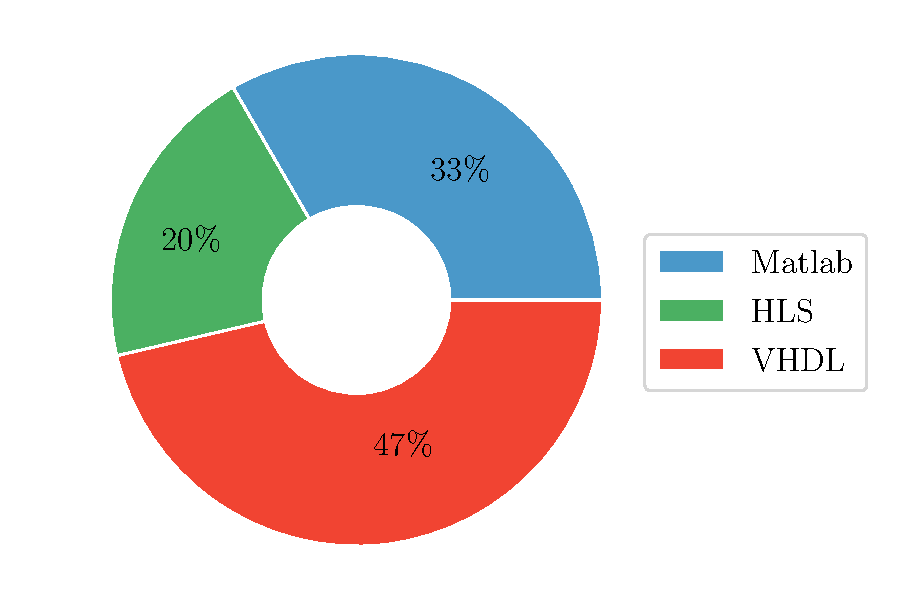
\includegraphics[trim=10 40 10 10,clip, width=0.65\textwidth]{img/matlab/lines_of_code_pie_chart_py_all} }}%
  \\
  %\hspace{\fill}
  \subfloat[\centering HLS in detail.]{{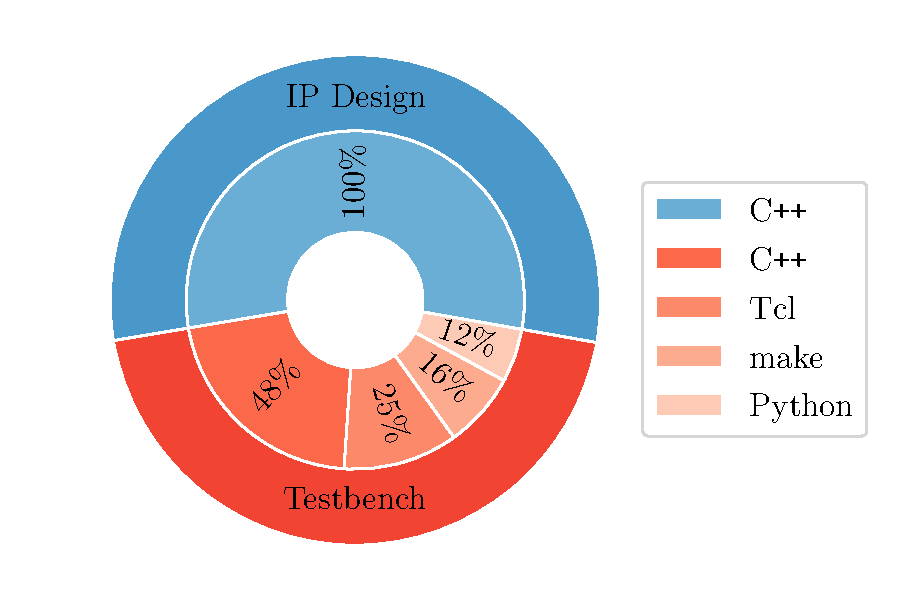
\includegraphics[trim=10 10 10 10,clip, width=0.49\textwidth]{img/matlab/lines_of_code_pie_chart_py_hls} }}%
  %\hspace{\fill}
  %\vspace{3cm}
  \subfloat[\centering VHDL in detail.]{{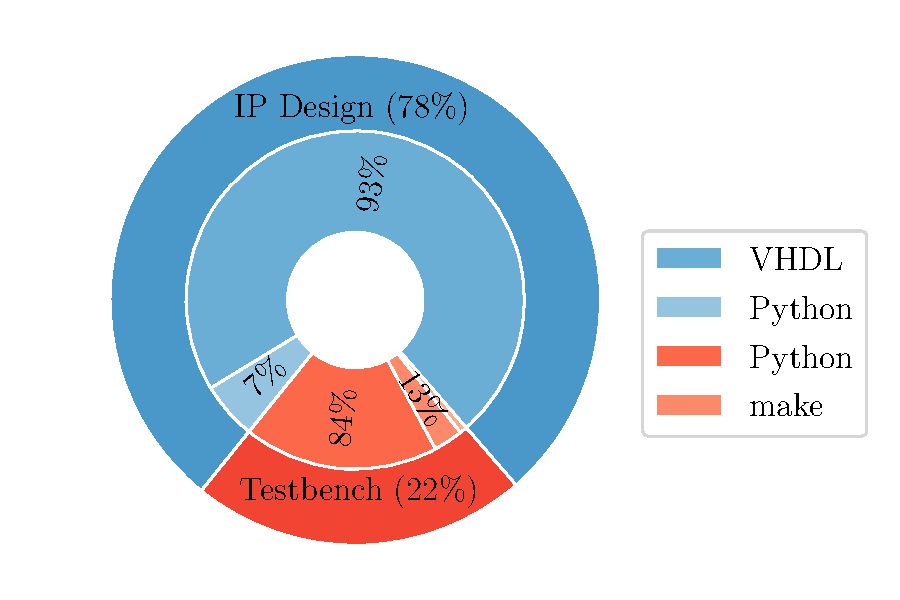
\includegraphics[trim=10 10 10 10,clip, width=0.49\textwidth]{img/matlab/lines_of_code_pie_chart_py_vhdl} }}%

  \caption{Lines of code of the respective code parts in the entire project, presented in multiple pie charts. The percentages of code in IP design and testbench for the HLS and VHDL implementations are shown in detail in the lower diagrams.}%
  \label{fig:lines_of_code_pie_charts}%
\end{figure}

\begin{table}[]
  \centering
  \begin{tabular}{l|c|c|}
  \cline{2-3}
  \textbf{}                                     & \multicolumn{1}{r|}{\textbf{IP Design}} & \multicolumn{1}{l|}{\textbf{Testbench}} \\ \hline
  \multicolumn{1}{|l|}{VHDL}                 & 3000                                    & 850                                     \\ \hline
  \multicolumn{1}{|l|}{HLS}                  & 920                                     & 740                                     \\ \hline
  \multicolumn{1}{|l|}{Common Testbench}        & \multicolumn{2}{c|}{630}                                                          \\ \hline
  \multicolumn{1}{|l|}{Matlab Model}            & \multicolumn{2}{c|}{2730}                                                         \\ \hline
  \multicolumn{1}{|l|}{Vivado Scripts}          & \multicolumn{2}{c|}{490}                                                          \\ \hline
  \multicolumn{1}{|l|}{\cplusplus\ Application} & \multicolumn{2}{c|}{2800}                                                         \\ \hline
  \end{tabular}
  \caption{The actual number of code lines for each code part, split in IP design and testbench, where applicable. All numbers are rounded up to tens.}
  \label{tab:lines_of_code}
\end{table}


%%%%%%%%%%%%%%%%%%%%%%%%%%%%%%%%%%%%%
\subsection{Implementation Time}

The metric of implementation time -- the time it takes to implement a specific feature -- is a subjective measure, since it heavily depends on the respective developer's experience, as already noted above.
In the present case, there is a strong background of knowledge and practical experience in VHDL design, while there is only very little of such in HLS design.
However, this metric is used in this section to specifically compare HLS with VHDL in this project.
Certain features are chosen for this comparison and their implementation times were logged during the actual implementation process.
The implementation is always considered as the HDL description, including the corresponding testbench code, to verify the respective correct functionality.
Table~\ref{tab:implementation_time_logging} shows the direct comparison between HLS and VHDL implementation times for these features.\\

\begin{table}[]
  \centering
  \begin{tabular}{l|c|c|}
  \cline{2-3}
                                                   & \multicolumn{2}{c|}{\textbf{Time [h]}} \\ \hline
  \multicolumn{1}{|l|}{\textbf{Feature}}           & \textbf{HLS}      & \textbf{VHDL}      \\ \hline
  \multicolumn{1}{|l|}{AXI Stream Interface}       & 8                 & 12                 \\ \hline
  \multicolumn{1}{|l|}{AXI4-Lite Interface}        & 2                 & 10                 \\ \hline
  \multicolumn{1}{|l|}{LED Control Register}       & 1                 & 2                  \\ \hline
  \multicolumn{1}{|l|}{Build Information Register} & 8                 & 5                  \\ \hline
  \multicolumn{1}{|l|}{Pass-Through Mode Register} & 1                 & 1                  \\ \hline
  \multicolumn{1}{|l|}{FIR Filter}                 & 13                & 7                  \\ \hline
  \multicolumn{1}{|l|}{Sample Decimation}          & 15                & 1                  \\ \hline
  \multicolumn{1}{|l|}{Receiver Structure}         & 13                & 33                 \\ \hline
  \multicolumn{1}{|l|}{\textbf{Sum}}               & \textbf{61}       & \textbf{71}        \\ \hline
  \end{tabular}
  \caption{Implementation time logging for a specific set of features, for the direct comparison between HLS and VHDL.}
  \label{tab:implementation_time_logging}
\end{table}

The following paragraphs present an insight into how the implementation times of the listed code parts arise.

%%%%%%%%%%%%%%%%%%%%%%%
\subsubsection{AXI Stream Inferface}

This is the main interface for the data input and -output of the DSP chain.
In HLS it can be automatically inferred by adding pragma directives to the respective function parameter variables.
Also the testbench code is implemented like a regular function call.
Therefore, the actual interface logic is completely hidden from the developer.
In VHDL on the other hand, this logic has to be implemented manually.
Also the testbench has to be hooked up with the correct signals and have a verificator logic, that supports the functional verification of an AXI stream interface.
Otherwise, this logic would have to be implemented manually as well.
In the time comparison, the larger amount of manual implementation in VHDL is clearly visible.
It is to note that this comparison does not compare functionally equivalent implementations, because the actually implemented logic in VHDL does not use the ready-flag correctly, as explained in the previous chapters.
According to this fact, a further increase in implementation hours should actually be considered for VHDL.
However, also the HLS implementation has its particular characteristics that need to be understood for a fully functional implementation.
Following the respective user guides and implementation examples provides a good starting point for that.

%%%%%%%%%%%%%%%%%%%%%%%
\subsubsection{AXI4-Lite Interface}

This interface is used to control IP settings and to read status information.
Similar to the previous AXI Stream interface, also this AXI4-Lite memory-mapped interface is automatically generated by HLS, while this has to be done manually in VHDL.
To create this process more efficiently and extendable, a Python script is used, which can also automatically generate VHDL code for the registers' memory map.
This turns out to be a multiplicator in productivity for the implementation of registers.
The register generator script was previously used in projects and is therefor already well-known and tested before it is used in this project.
However, the VHDL code only represents one part of the interface -- the second part is the firmware driver that is used in the application software.
Even though the register generator script also generates a \cplusplus\ header file that includes several address offset definitions of the registers, the actual driver functions need to be implemented manually.
Several files need to be integrated into a pre-defined folder structure, in order to enable a correct integration of the IP in a Vivado block diagram.\\

Again, the amount of manual steps in the VHDL implementation are clearly represented in the number of hours that are spent.

% TODO: mention figure out of read-only and read-write types (pointer/reference)
% TODO: mention testbench (vhdl: support block, hls: simple access to variable)

%%%%%%%%%%%%%%%%%%%%%%%
\subsubsection{Registers}

Once the AXI4-Lite memory-mapped interface's main functionality is implemented, further registers can be added.
In the specific implementation for this project, registers for LED control, the DSP mode, as well as a build information register are added.
The latter holds information about the build date and -time of the IPs, and is particularly time-consuming because of the implementation of the respective drivers to convert the date format in both variants.
In contrast, the addition of the LED control and DSP mode registers is simple and fast, because of the auto-generated code in HLS and VHDL with usage of the register engine.
The single bits in the LED control register directly represent the LEDs' values on the hardware.
The DSP mode register can select the regular FM radio mode and a pass-through mode, which simply forwards the streaming data without any processing.
Summing up, the addition of registers to the design can be time-consuming in both variants, depending on the required driver functionality.
However, the general tendency is that VHDL requires more time, because of this driver issue.

%%%%%%%%%%%%%%%%%%%%%%%
\subsubsection{FIR Filter}

The FIR filter is one of the main DSP blocks of the design, as it is used in multiple instances throughout the design.
Therefore, its implementation was done with special care, in order to guarantee its correct functionality.
Consequently, a unit test is implemented in the testbench, which is also included in the listed number of implementation hours.\\

For the \cplusplus\ version, a code example for an FIR filter, which is provided by Xilinx HLS, is taken and modified for the present purpose.
The VHDL variant is taken from an older DSP project, which was previously developed during a university course.
However, the integration and testbench code is developed for this project, specifically.
Here, the HLS implementation took significantly longer, because of the limited knowledge regarding the usage of an AXI stream interface.
It is the first time in the project, that this type of interface is applied in the IP design and used in the testbench.
The VHDL implementation was straightforward in comparison.
The testbenches compare the FIR filters' output with the Matlab model's pilot tone output.
Both variants match the output results of the Matlab model successfully.

%%%%%%%%%%%%%%%%%%%%%%%
\subsubsection{Sample Decimation}

The implementation of the sample decimation functionality differs slightly between the two variants, HLS and VHDL.
This is explained in Section~\ref{sec:impl:hls:sample_rate_reduction}.
The implementation time of the HLS version is severely larger than the VHDL version.
This is mainly due to the limited knowledge of the functionality of the AXI stream interface at this stage in the project's implementation, just as previously mentioned with the FIR filter.
The initial version was implemented like the VHDL version -- a counter that only triggers the subsequent DSP blocks upon a certain number of samples was received.
However, this led to an endlessly blocking AXI stream in the testbench execution.
The reason was, that the read-function can only read a sample when the respective stream contains a sample, and that it is a blocking function.
Because the sample decimator did not write a sample every time, the subsequent read-function blocked indefinitely.
A thorough investigation in several user guides, in combination with step-by-step debugging, the issue was found and led to the current, working implementation, which processes a number of samples, before it forwards one sample.
The process of finding this issue explains the largely varying implementation times, as listed in Table~\ref{tab:implementation_time_logging}.

%%%%%%%%%%%%%%%%%%%%%%%
\subsubsection{Receiver Structure}

The implementation of the receiver structure requires the combination of several previously implemented blocks, such as the FIR filter and any interfaces.
This is done according to the Matlab model, to resemble its functionality.
The VHDL version is significantly more time consuming in comparison to HLS.
However, it is to note at this point that the VHDL version is implemented first, and thus some issues are already solved by the time of the HLS implementation.
Nevertheless, the VHDL implementation takes longer, as it requires more detailed care in the signal level.
This specifically includes the clock-alignment of any signals that need to be used in a combination.
For example, if two parallel FIR filters produce output signals that are to be added, they need to be aligned so that they are valid at the time of the summation.
This often requires analysis and debugging in a signal wave form.
In HLS this is not required, since the validity of a signal is determined internally by the HLS compiler, according to the usage of the respective data variables.
Another factor that adds up to the implementation time is the number of lines of code, as presented in Table~\ref{tab:lines_of_code}.
The VHDL IP design requires 3000 lines, while the HLS IP design only takes 920 for the same functionality.
Again, this is a subjective measure -- several factors such as code style, or the developer's experience play a role -- but still shows a good representation of the implementation effort for this project.\\

In the final summation over several implementation times of all the listed features, the two variants HLS and VHDL only differ by 10 hours, which is around 15\%.
However, as the previous paragraphs explain, prior knowledge regarding HLS was limited and had to be gathered during the ongoing implementation.
Nevertheless, even consiering this fact, the HLS implementation is faster than the VHDL equivalent.
Thus, with an equal amount of prior knowledge and experience, it is assumed that an HLS implementation can lead to a successfully functioning result significantly faster.


% Implementation effort/time
%    -- see logged times; is subjective; had no previous knowledge
%    -- AXI interfaces --> huge effort in VHDL...
%        (mention Johannes Walter for generously providing/allowing the Register Engine script, adapted for this thesis)
%    -- drivers are auto-generated with HLS! huge time-saving..
%       (maybe show the code of AXI4-Lite interface and its generated driver
%        --> difference between R/W and RO!;
%        and show screenshots of the IP in the block design)

% Issues
% -- HLS Debug Error with Bitwidth:
%       Not sure what the error was.
%       Parallel delay for I/Q didn't work.
%       The order of every 2nd data value was wrong.
%       Using a single delay fixed it.
% -- HLS driver generation
%       Fixing issue with auto-generated driver.
%       It did not get imported into the SDK.
%       Problem was that HLS project and top-level
%       did not have the same name....

%%%%%%%%%%%%%%%%%%%%%%%%%%%%%%%%%%%%%%%%%%%%%%%%%%%%%%%%%%%%%%%%%%%%%%%%%%%%%%
\section{Simulation Speed}

In this section, the simulation speed of the multiple implementation variants in their various abstraction levels are compared.
Simulation speed in this context refers to the number of input samples that the DUT can process in a time unit, like one second.
In the current application, the antenna signal is recorded and replayed to the DUT in the simulation.
This ensures a reproducable result, so that the different variants can be compared against each other reliably.\\

Figure~\ref{fig:impl_time_analysis} shows this direct comparison of processed samples per second for the implementation variants.
The measurements always include the testbench setup-phase, and the run-phase.
The setup-phase mainly consists of loading the recorded data and its preparation, so that it can be fed into the DUT.
The run-phase then actually applies this test data to the DUT and stores the respective output results.
All time measurements are taken without the result analysis, since this is the exact same, shared code between all variants and thus takes the same amount of time everywhere.
Several measurements are done multiple times, to achieve an average result, that is independent of the current processor load of the host PC.\\

The diagram shows an immense difference of simulation speed between the variants.
It is important to note that the y-axis has a logarithmic scale, as a method to enable the presentation of the values in multiple orders of magnitude.
VHDL only achieves around 20 samples per second.
This is by far the slowest method, which is expected because of the way of how VHDL is simulated.
This can not be explained in detail here, but one main feature of a VHDL simulator is its capability to simulate parallel processes, as they occur in actual parallel hardware.
The VHDL simulator therefor needs to evaluate several concurrent processes and statements, whenever any of the interacting signals change their value, and this is time-consuming.
In the current case, there is an additional interface between the VHDL simulator and the Python testbench framework, which likely additionally slows down the simulation.
The HLS testbench in comparison achieves around 50000 samples per second, which is a speed-up factor of 2500.
This is specifically talking about the HLS C/\cplusplus-simulation.
The main reason for the speed-up therefor is, that in this type of simulation no timing behaviour is simulated -- any processes are treated as C/\cplusplus\ functions that runs like a regular executable on the host CPU.
Also, the HLS compiler is using native \cplusplus\ data types to represent the signals, where possible, which results in the faster execution of the code.
Finally, the simulation in Matlab achieves a further speed-up by a factor of 70.
Matlab is specifically designed for applications which require matrix calculations and utilizes highly optimized algorithms in its underlying functions therefor.
Thus, Matlab runs very efficiently and achieves the highest simulation speed of around 3 million samples per second.

%
% VHDL:
%          time                   samples
%   audio         sim           in      out
%  0.1000 s    73:44 min       96000 -> 4000
%  0.0100 s    09:37 min        9600 ->  400
%  0.0025 s    02:36 min        2400 ->  100
%
% HLS:
%          time                   samples
%   audio         sim           in      out
%     0.8 s    00:17 min       768000 -> 32000
%     1.7 s    00:36 min      1632000 -> 68000
%
%
% Matlab:
%          time                   samples
%   audio         sim           in      out
%     1.7 s  00:00:00.52 min   1632000   68000
%

\includepicture [0.55] [0, trim=10 10 10 10, clip] {The measured simulation speed of the different implementation variants, in samples per second. The arrows show the speed-up factors. Note the logarithmic scale of the y-axis.} {impl_time_analysis} {img/matlab/impl_time_analysis}


%%%%%%%%%%%%%%%%%%%%%%%%%%%%%%%%%%%%%%%%%%%%%%%%%%%%%%%%%%%%%%%%%%%%%%%%%%%%%%
\section{System Design}

The system design architecture that is chosen in this project covers several parts of the system.
This includes a reference model, the development of the IP itself, including the simulation testbench, as well as the final integration into the productive system.
Because of this modular and structured approach, that is given by this system design, it can be applied to almost any DSP project.
The main processing IP can simply be replaced with another implementation, while the environment does not need to be modified.
The reason therefor is, that DSP projects almost always use streaming interfaces for their inputs and outputs.
Also a configuration interface is commonly used, to adapt certain parameters of the IP during runtime.


%%%%%%%%%%%%%%%%%%%%%%%%%%%%%%%%%%%%%%%%%%%%%%%%%%%%%%%%%%%%%%%%%%%%%%%%%%%%%%
\section{Deployment on Hardware}

The VHDL and HLS implementation variants are implemented, simulated in their testbenches to verify the correct functionality, as well as deployed on hardware, to test their performance in an actual application.
Important parts of this end-to-end integration are presented here.

%%%%%%%%%%%%%%%%%%%%%%%%%%%%%%%%%%%%%
\subsection{Integration}

The aim is to create IP blocks, that can be integrated into a block design in the Xilinx Vivado software.
The IP blocks should be able to be connected with their AXI interfaces, in order to successfully communicate and interact with the embedded hard-processor, the ARM CPU.
In the case of HLS, several files that are required for this integration are generated automatically.
The files are already placed into the specific folder structure, that Vivado requires to recognize it as an IP block.
In the case of VHDL on the other hand, this needs to be done manually.
There is an assistant, the IP Packager, which helps the developer to create the IP.
However, at this point the folder structure already needs to be in place, so that the assistant works correctly, which again requires manual action.
Regarding the top-level interfaces, the IP Packager supports an auto-detection of the signals that belong to the respective interface types, as long as they follow the expected naming guidelines.
However, the interface itself needs to be defined and updated manually in the IP Packager.
This is especially important, if the interfaces change in the VHDL code.\\

However, also the auto-generation of the HLS IP has characteristics that require special attention.
One issue during the implementation was, that the auto-generated software driver did not get imported into the Vivado SDK.
The reason therefor was, that the top-level function of the IP did not have the exact same naming as the Vivado HLS project.
For issues like that, the Eclipse-based SDK does not give any error output or any kind of information.
This however is a general issue with the SDK, where error handling is poor and error log outputs are not existent, or at least not useful to the developer, so that the SDK sometimes crashes without an obvious reason.
It is to note, that version v2018.2 is used for the entire Vivado toolchain, which is not the latest version that is currently available.
Thus, some of the occuring issues may already be fixed in the newer versions.\\

However, both IPs could successfully be integrated into the Vivado block design, and the tests on the hardware show that they function correctly within the system.

%%%%%%%%%%%%%%%%%%%%%%%%%%%%%%%%%%%%%
\subsection{Hardware Utilization}

The hardware utilization of the HLS and VHDL implementations are compared in detail in this section.
The numbers are taken from the final utilization report, that is created by Vivado at the end of the bitstream creation, since this is assumed to be the most accurate report that shows the actual utilization.\\

Figure~\ref{fig:hardware_utilization} shows the utilization numbers of the different FPGA resources.
It reveals that the manual VHDL implementation clearly requires more resources in the FPGA.
The study of the detailed utilization report however does not enable a deeper direct comparison of the respective single blocks, such as VHDL FIR filter against HLS FIR filter.
This is because the HLS compiler automatically applies optimizations, so that the direct connection between code and resource report is partially lost.
Examples for optimizations are inlining of functions, re-ordering of operations and time-sharing.
The latter has an especially large impact on the resource utilization.
Generally, in hardware design there is a trade-off between resource utilization and throughput, which leads to time-sharing.
For example, an entirely parallel-duplicated pipeline can process the double amount of data, but also requires the double amount of resources.
On the other hand, time-sharing a resource may take the double amount of time, thus only processes half of the data, but also only requires half of the resource utilization.
In HLS, this trade-off can be influenced and determined by the developer.
Depending on the requirements of the design, the optimization may either be set towards a lower resource utilization, or towards a high throughput.
In the current HLS implementation, no measures are taken towards any optimization and thus, the compiler is free to decide.
However, the only requirement is the correct functionality within the given situation, of course.
This specifically means that the throughput needs to be high enough, in order to process the audio signal output accordingly.\\

Nevertheless, the resource report allows the comparison of the configuration interface, which is the AXI4-Lite interface.
In VHDL, it requires 44 LUTs and 54 FFs, while HLS consumes only 36 LUTs and 37 FFs.
So it seems that the manual VHDL implementation requires more resources in all the comparable parts.
By further investigating the report, the VHDL version apparently utilizes a large amount of LUTs for the delays, which are used to clock-align the FIR output signals.
For an optimization of the VHDL design, this would be a good point to start at.
However, for this project, both implementation variants are compared without any optimizations from the developer's side.


\includepicture [0.75] [0, trim=10 10 10 10, clip] {A comparison of the resource utilization of the VHDL and HLS implementations. The VHDL variant requires significantly more resources.} {hardware_utilization} {img/matlab/hardware_utilization}

%%%%%%%%%%%%%%%%%%%%%%%%%%%%%%%%%%%%%
\subsection{Latency}

Latency is the time it takes for the design to produce an output sample.
The latency of the HLS version is taken from the report that is produced after the C-synthesis of the HLS compiler.
The report shows an estimated resource utilization, as well as the latency as a number of clock cycles.
The latency is given with 2712 clock cycles.
For the VHDL version, a similar report is not available.
Instead, the testbench of the integration test is executed, which produces a signal wave form.
The latency is measured from this wave form and results in a number of 2470 clock cycles.
With regards to latency, the two implementation variants appear to have a similar behaviour.


%%%%%%%%%%%%%%%%%%%%
\chapter{Conclusion and Prospect}
\label{cha:ConclusionAndProspect}

This thesis covers a comprehensive variety of topics, that ranges from digital signal processing to system modeling and -design, IP design in different methods, verification, to hardware-software interaction in hardware.
The implementation of the FM radio receiver in multiple different methods, namely GNU Radio, Matlab, VHDL and HLS so that they achieve the same functionality, is a challenge, especially with the latter methods.
However, this challenge is solved within an end-to-end system design, that strongly supports the development process.\\

GNU Radio is a software, that allows an efficient development of a software-defined radio as a prototype, which can run on actual hardware in a live environment.
It is definitely worth to use it during the development of a project like the one in this thesis, since it allows to achieve a functioning result with relatively low effort.\\

The usage of Matlab as a tool to research DSP algorithms and strategies to demodulate a signal, in order to ultimately find a system model that can be implemented in hardware, turns out to be a powerful asset.
It allows the development in fast iterations, through short simulation times, to achieve a result quickly.
Based on this system model, the implementation of actual hardware IPs, with VHDL and HLS can be done more efficiently and in a direct way, because issues in the algorithm level are already fixed in the model at this point.
In combination with the simulation testbenches that share major parts, such as the input source, as well as a the analysis tool, the IP development works smoothly and efficiently.
The verification as a comparison against the Matlab system model gives instant feedback of whether the IP functions correctly.
Even if the system model changes, the testbench automatically adapts, since the input source files are re-generated by the model and thus picked up at the next iteration of the testbench simulation, so the hardware engineer can also adapt the IP code.
Once the IP is deployed on actual hardware, it is tested by the firmware, in order to check its correct functionality again, which closes the loop from the system model and the IP simulation to the hardware deployment.
This entire process proved itself to be a successful approach.\\

Regarding the implementation of the VHDL and HLS IPs and the accompanying comparison, the result turns out to be unexpected.
The initial expectation, that HLS is inefficient in terms of resource utilization, is contradicted.
Also the amount of time spent in the implementation and the metric of lines of code create a positive picture of HLS.
Further, the automatic generation of several files that are required to integrate the IP into a system design, such as interface definitions or software drivers, support this attitude.
VHDL may have its advantages in specific areas of application, but HLS is definitely a powerful tool that can achieve great results in less time.
This is especially true, when it comes to the development of complex functionalities, such as image- or video processing, with the support of built-in libraries like OpenCV.





% NOTES:
%
% Further steps:
%  - generate VHDL from Matlab receiver code
%  - use the common input file and feed it to GNU Radio;
%    also produce an output file with GNU Radio for comparison
%  - Develop HLS compiler independent code (optional)}
%    -- Different compilers use different #pragmas, etc.
%    -- These #pragmas need to be within the code, at the appropriate positions,
%       which makes it difficult to write compiler independent code....
%  - use Matlab Simulink HDL Coder and System Generator
%     as additional implementation variants
%  - use Intel oneAPI HLS compiler
%      -- try to develop compiler-independent code
%      -- how platform-independent is HLS?
%  - explore HLS optimizations
%  - explore HLS libraries (e.g. DSP library --> pre-made FIR filter)
%  - create another IP in the same system
%      -- due to the modular system design this is easy to do
%  - use Linux OS on the SoC, to enable live-data streaming with the RTL-SDR
%
%
%
% ...the list shows how comprehensive the topic of this thesis is.
% Based on the results that were made during the elaboration, many more ideas came into play.
% Many ideas to extend the project, ...

%%%%%%%%%%%%%%%%%%%%%%%%%%%%%%%%%%%%%%%%%%%%%%%%%%%%%%%%%%%%%%%%%%%%%%%%%%%%%%
%\section{Advantages / Disadvantages}

easy and much faster to get complex HDL code, such as image/video processing, through libraries like OpenCV.\\
A developer still needs to have a strong hardware background, to be able to understand what is being generated in hardware from x lines of code in HLS/Cpp.



%%%----------------------------------------------------------
\appendix                                         % appendix
%%%----------------------------------------------------------

\chapter{Supplementary Materials}
\label{app:materials}


A list of supplementary data, that is included with this thesis.

\section{PDF Files}
\begin{FileList}{/}
\fitem{thesis.pdf} Master thesis
\end{FileList}

\section{FM Radio Receiver Project}
\begin{FileList}{/fm-radio}
\fitem{/doc} Documentation, Analysis tools and this thesis document.
\fitem{/hardware} Hardware development, HLS and VHDL.
\fitem{/sim} Simulation, including GNU Radio and Matlab.
\end{FileList}

\vspace{5 mm}
\noindent
The FM Radio Receiver project can also be found on GitHub:\\
\url{https://github.com/wurmmi/fm-radio}

	% contents of the CD-ROM/DVD

\backmatter
\chapter{List of Abbreviations}
\label{cha:listabbrev}

\begin{tabbing}
\hspace{25 mm}\=\kill

\textbf{ADC}       \> Analog Digital Converter\\
\textbf{AM}        \> Amplitude Modulation\\
\textbf{AXI}       \> Advanced Extensible Interface\\
\textbf{BP}        \> Bandpass (Filter)\\
\textbf{CI}        \> Continuous Integration\\
\textbf{DC}        \> Direct Current\\
\textbf{DSB-SC}    \> Dual-Sideband Suppressed-Carrier\\
\textbf{ERP}       \> Effective Radiated Power\\
\textbf{FM}        \> Frequency Modulation\\
\textbf{FPGA}      \> Field-programmable Gate Array\\
\textbf{HLS}       \> High-Level Synthesis\\
\textbf{IF}        \> Intermediate Frequency\\
\textbf{IoT}       \> Internet of Things\\
\textbf{IP}        \> Intellectual Property\\
\textbf{IQ,I/Q}    \> Inphase and Quadrature components\\
\textbf{LED}       \> Light Emitting Diode\\
\textbf{LP}        \> Lowpass (Filter)\\
\textbf{LNA}       \> Low Noise Amplifier\\
\textbf{LO}        \> Local Oscillator\\
\textbf{PM}        \> Phase Modulation\\
\textbf{RTL}       \> Register Translation Level\\
\textbf{SDR}       \> Software Defined Radio\\
\textbf{SoC}       \> System On Chip\\
\textbf{VHDL}      \> Very High Speed Integrated Circuit Hardware Description Language\\
\textbf{VHF}       \> Very High Frequency\\

\end{tabbing}


%\addcontentsline{toc}{chapter}{\listfigurename}
%\listoffigures

%%%----------------------------------------------------------
\MakeBibliography                        				% references
%%%----------------------------------------------------------

%%% special page for checking print size --------------------
\chapter*{Check Final Print Size}

\begin{center}
{\Large --- Check final print size! ---}

\bigskip

\calibrationbox{100}{50} % width/height of box in mm

\bigskip

{\Large --- Remove this page after printing! ---}

\end{center}



%%%----------------------------------------------------------
\end{document}
%%%----------------------------------------------------------
